\typeout{NT FILE related_work.tex}%
\glsresetall
\chapter{Background and Related Work}
% \label{cha:introduction}

In this section, we present the background required for the understanding and the conception of our solution. We also discuss the current state-of-the-art graph processing frameworks we considered relevant and that can be used for comparison against our solution.

We start by presenting some basic notions about the architecture and execution model of the \gls{GPU}, as well as the most famous and best performing \gls{GPU} programming model named \gls{CUDA}~\cite{paper:cuda}. 
%
We then present the Marrow framework and give a brief detailing of its inner workings. 
%
Finally, we study how graphs can be stored and processed on the \gls{GPU}. To this end, we present the various data structures that can be used to represent graphs, the existing programming models to process graphs, and the existing state-of-the-art high-performance graph processing frameworks.

\section{GPU}

The most common usage of the \gls{GPU} is to render images intended for output to a display device. However, these chips can also be used for any generic computations
%, given that they are turing complete just like a regular \gls{CPU}
. Using a \gls{GPU} for other types of computations besides image rendering is known as \gls{GPGPU}. The main difference between a \gls{GPU} and \gls{CPU} lies in their core count and complexity. \gls{GPU}s contain thousands of "low" frequency (around 1 to 3 GHz) and low complexity compute cores, while \gls{CPU}s typically have between 1 to 32 cores with a high frequency (around 2 to 6 GHz) and high complexity. This type of architecture makes \gls{GPU}s the ideal platform for highly parallelizable applications~\cite{paper:cuda}. \gls{CPU}s are designed to achieve a good performance in a wide variety of tasks. To this end, the \gls{CPU}'s design is aimed at minimizing latency, having a powerful arithmetic logic unit, big caches, and utilizing techniques like branch prediction and data forwarding. The \gls{GPU}'s design, on the other hand, is aimed at maximizing efficiency, leveraging large numbers of efficient compute units, arithmetic logic units, and pipelining~\cite{site:nvidiaCudaGuide}.

\subsection{Architecture}

\begin{figure}[tbp]
  \centering
    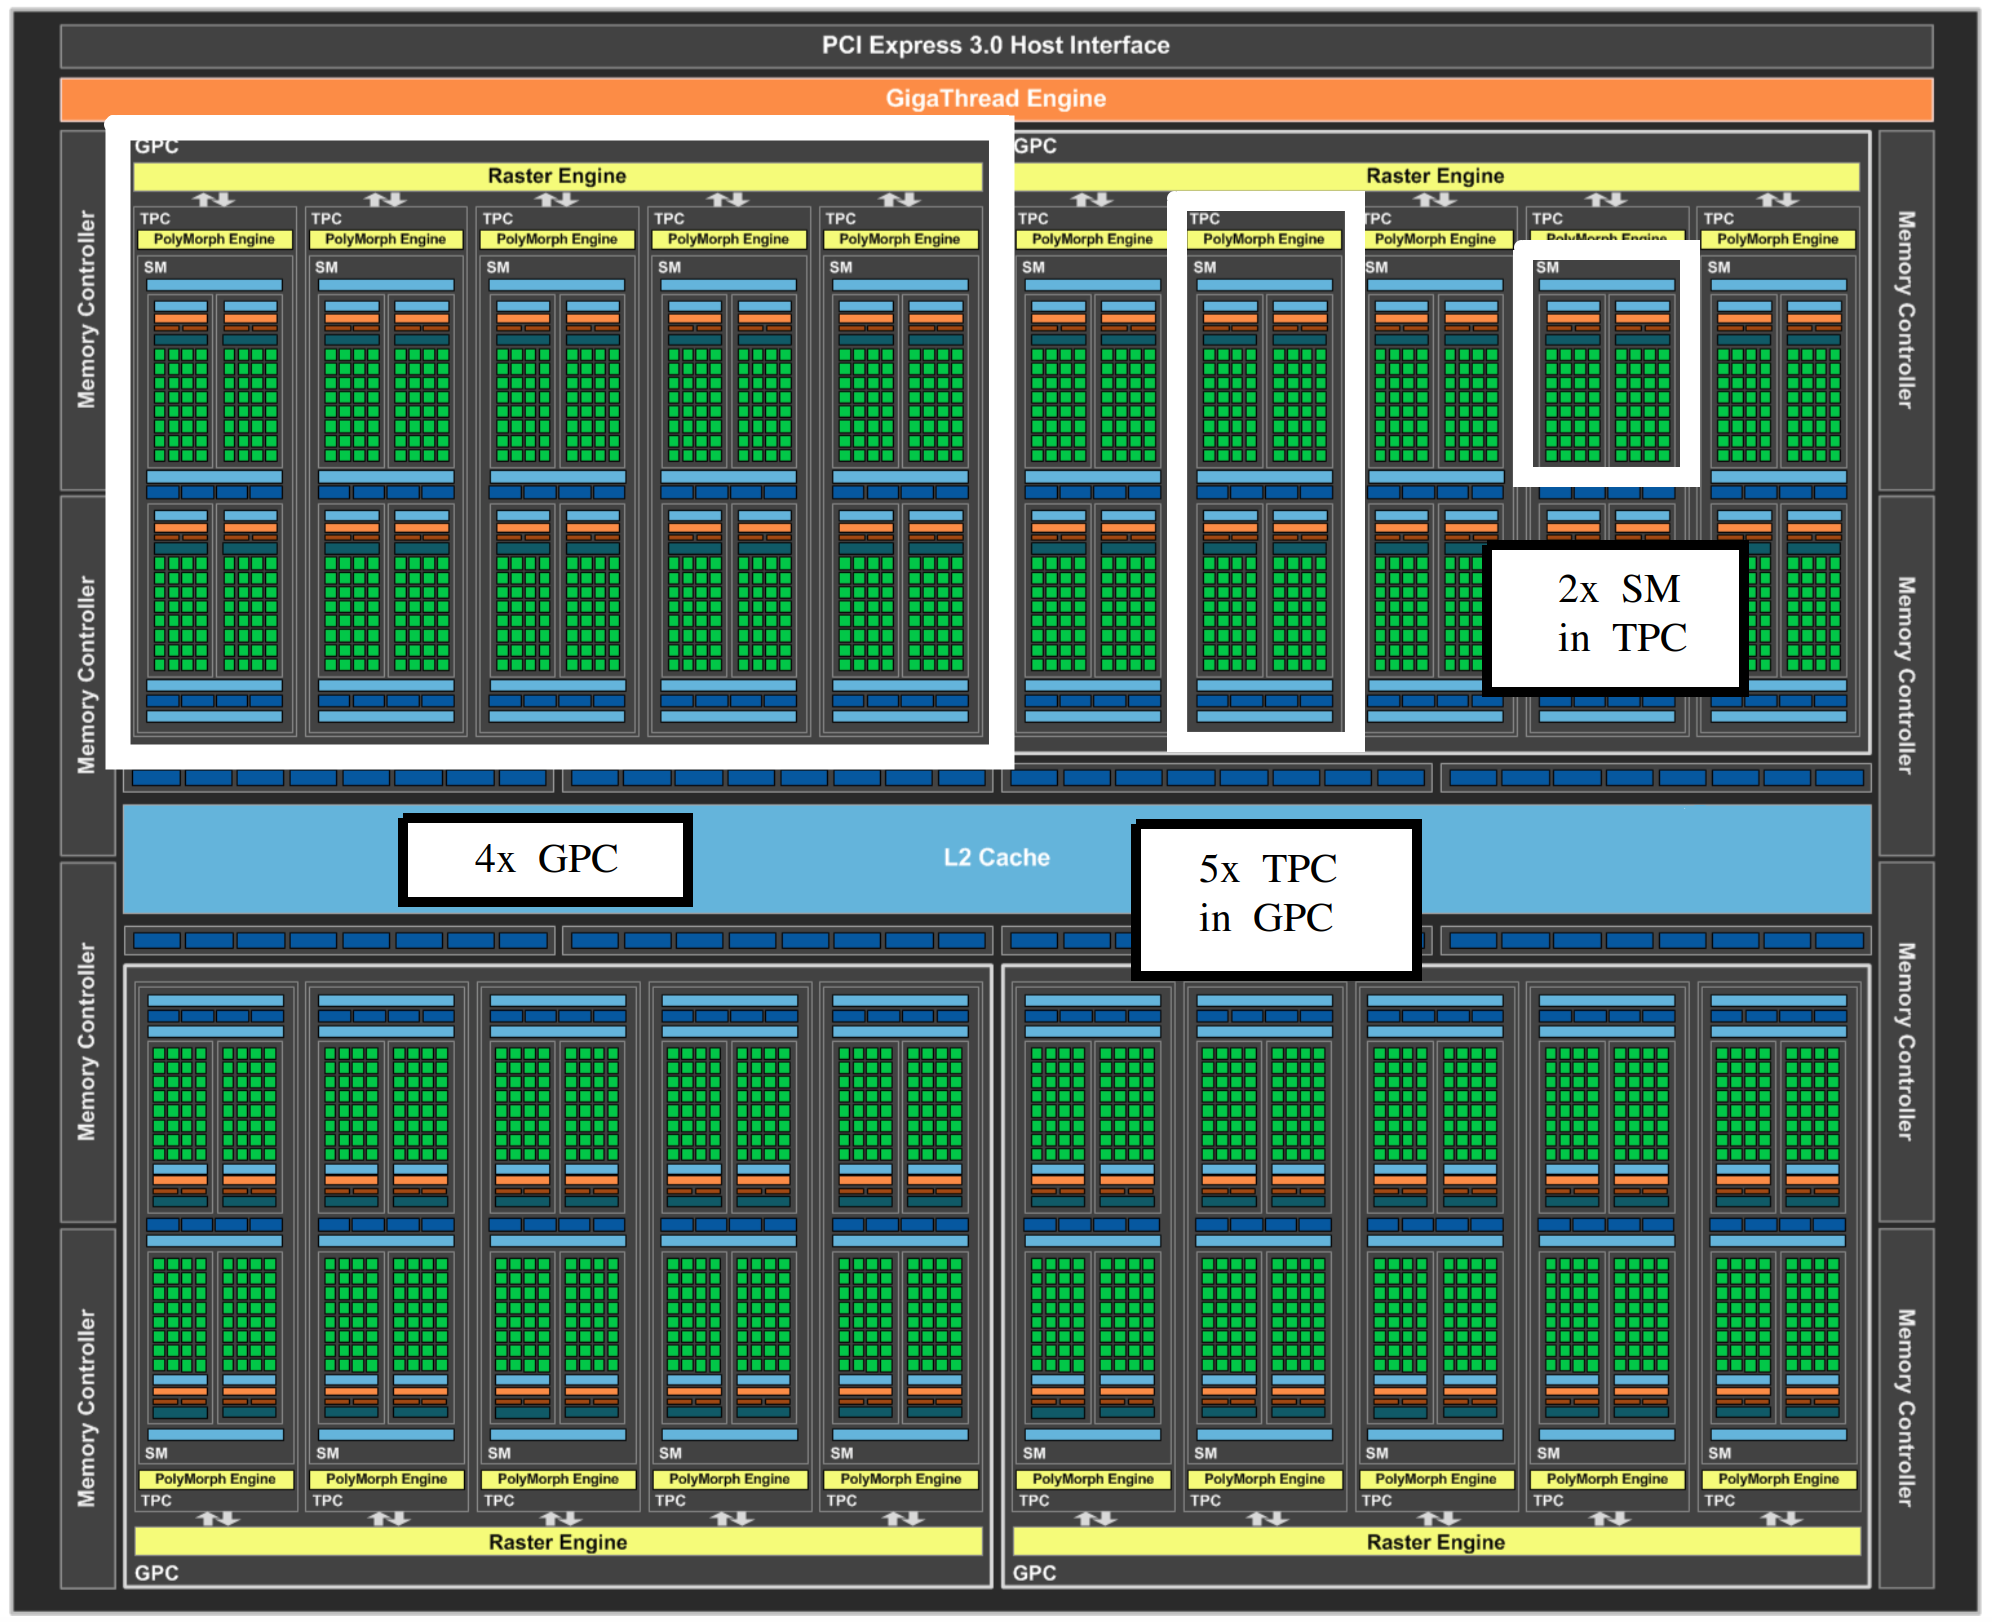
\includegraphics[width=0.85\textwidth]{Chapters/Figures/Images/pascal_labeled.png}
    \caption{GP104 Pascal Architecture with 40 \gls{SM} units}
\label{fig:pascal}
\end{figure}

% \begin{figure}
% \label{fig:sm}
%   \centering
%     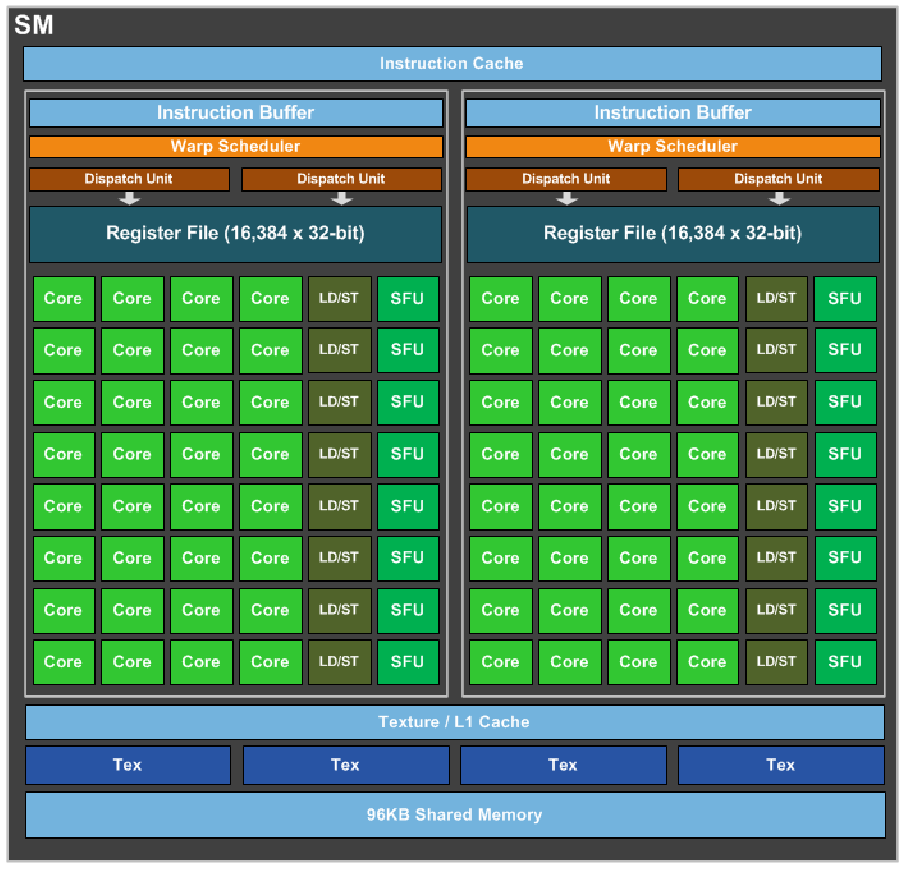
\includegraphics[width=0.65\textwidth]{Chapters/Figures/Images/sm_2.png}
%     \caption{Pascal Stream Multiprocessor}
% \end{figure}

Given that we will be working with the \gls{CUDA} interface, which only supports Nvidia \gls{GPU}s, we will focus on the architecture of Nvidia graphics cards, specifically the Pascal architecture\footnote{More modern Nvidia architectures are more complex containing, for example, dedicated Tensor Cores for machine learning purposes which are not directly relevant for this work.}. It should be noted, however, that a lot of  these concepts are also applicable to architectures from other \gls{GPU} manufacturers.

As seen in Figure~\ref{fig:pascal}, the \gls{GPU} is divided into multiple \gls{GPC}s, which contain multiple \gls{TPC}s, which typically contain two \gls{SM}s plus memory controllers. Each \gls{SM} 
%(Figure~\ref{fig:sm}) 
is composed of compute cores, special function units, double precision units, and other specialized units. The \gls{SM}'s main purpose is hosting the execution of warps of 32 threads. These will be addressed in more detail in section~\ref{sec:execution_model}~\cite{whitepaper:gtx1080, whitepaper:pascal}.

The memory in a \gls{GPU} can be divided in two categories, device memory and on-chip memory. The device memory is a global high-bandwidth \gls{DRAM} memory. This memory has a high capacity but also high latency, in the order of hundreds of clock cycles. On-chip memory is composed of shared memory registers, constant memory, L1 and L2 caches, and texture caches. Threads running in the same \gls{SM} have access to a shared memory, meaning that memory accesses to shared memory within a \gls{SM} are faster than accesses to global memory but slower than accesses to local memory. Shared memory within a \gls{SM} has a very limited capacity, in the order of dozens of kilo-bytes~\cite{survery:graph_processing_on_gpu}.

\subsection{Execution Model}
\label{sec:execution_model}

When doing \gls{GPGPU}, we usually refer to our main system as the host, and our accelerator as the device. The host configures and sends kernels to the device, and also transfers and allocates data between the two. The device executes the kernels specified by the host.

A kernel is essentially a function that is executed using a grid of blocks of threads on the device. Each block is executed by a \gls{SM} and each thread is executed by a \gls{SM}'s core. All threads execute the same instructions and have access to their thread ID (ID within a block), block ID, and the dimensions of the grid. These IDs are used to select the correct data to process and make control decisions. in Figure~\ref{fig:grid} is an example of such a grid. These grids are defined by the programmer and can have between 1 and 3 dimensions (both the block layout and thread layout within the blocks), which impact how the IDs of both the blocks and threads are distributed~\cite{survery:graph_processing_on_gpu}. Block sizes have limits that differ from architecture to architecture (Ex: 1024 x 1024 x 64).

Once a kernel is invoked, the \gls{GPU} assigns each block to a \gls{SM} (hardware is free to assign blocks to any \gls{SM}), where each \gls{SM} can handle multiple blocks. Blocks are in turn executed using warps (units of 32 threads). These warps execute in lock-step and with no order guarantees, meaning that all threads within a warp execute the same instruction in each clock cycle, but there are no guarantees in which order the warps will be executed. To improve performance, if a given warp has to execute an expensive operation, like reading from global memory, a \gls{SM} can start executing operations from another warp while the previous awaits for a result~\cite{site:nvidiaCudaGuide}. This technique is called latency hiding.

\begin{figure}
  \centering
    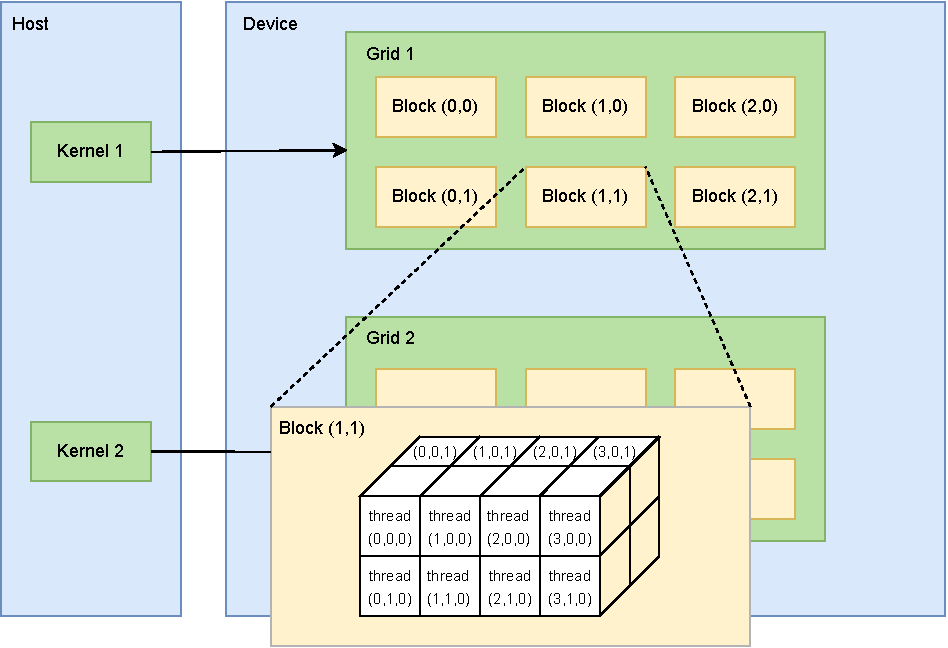
\includegraphics[width=0.75\textwidth]{Chapters/Figures/Images/grid.pdf}
    \caption{Grid with 3D blocks (adapted from diagram in~\cite{site:cudablog})}
\label{fig:grid}
\end{figure}

\section{CUDA}

\begin{listing}%[tbp]
\begin{minted}
[
frame=lines,
linenos,
fontsize=\scriptsize
]
{cpp}
#define N 2048
#define THREADS_PER_BLOCK 512
__global__
void add(int* res, int* b, int* c, int n) {
    int index = threadIdx.x + blockIdx.x*blockDim.x;
    if(index < n)
        res[index] = b[index] + c[index];
}

int main() {
    int *res, *b, *c;
    int *d_res, *d_b, *d_c; // Device data
    int size = N * sizeof(int);
    
    // Allocate and init host data
    b = (int*)malloc(size);
    c = (int*)malloc(size);
    res = (int*)malloc(size);
    init_data(b, c, N);
    
    // Allocate device data
    cudaMalloc((void**)&d_b, size);
    cudaMalloc((void**)&d_c, size);
    cudaMalloc((void**)&d_res, size);
    
    // Copy data from host to device
    cudaMemcpy(d_b, b, size, cudaMemcpyHostToDevice);
    cudaMemcpy(d_c, c, size, cudaMemcpyHostToDevice);
    
    // Specify grid and invoke kernel
    long nb = (N+THREADS_PER_BLOCK-1)/THREADS_PER_BLOCK;
    add<<<nb, THREADS_PER_BLOCK>>>(d_res, d_b, d_c, N);
    
    // Copy result data from device to host
    cudaMemcpy(res, d_res, size, cudaMemcpyDeviceToHost);
    
    // Deallocate memory
    cudaFree(d_b); cudaFree(d_c); cudaFree(d_res);
    free(b); free(c); free(res);
}
\end{minted}
\center
\caption{Vector addition in \gls{CUDA}.}
\label{lst:cuda-add-vecs-main}
\end{listing}

The most popular and best performing \gls{GPGPU} programming model is Nvidia's \gls{CUDA}. Within a C++ program, \gls{CUDA} allows us to transfer data between the host and device, specify a kernel using an annotated function, and invoke it specifying the layout of the associated grid. A typical \gls{CUDA} program is composed by the following steps:

\begin{itemize}
    \item Allocate and initialize data on the host.
    \item Allocate memory on the device.
    \item Copy data from the host to device.
    \item Specify the grid layout and invoke a kernel defined using an annotated function that has access to a \texttt{threadIdx}, \texttt{blockIdx}, and \texttt{blockDim}.
    \item Copy result data from device to host.
    \item Deallocate memory.
\end{itemize}

Listing~\ref{lst:cuda-add-vecs-main} provides an example of such a program that adds two vectors on the device. Matrices \texttt{b}, \texttt{c} and \texttt{res} are allocated and initialized on the host. Then matrices \texttt{d\_b}, \texttt{d\_c} and \texttt{d\_res} are allocated on the device, and \texttt{b} and \texttt{c} are copied to \texttt{d\_b} and \texttt{d\_c} respectively. The kernel \texttt{add} is invoked using a grid with \texttt{nb} blocks and \texttt{THREADS\_PER\_BLOCK} threads in each block. Note that we round up the number of blocks \texttt{nb} in line 31. The grid dimensions are specified within the $\lll \ggg$ delimiters. In the \texttt{add} kernel, the \texttt{threadIdx} and \texttt{blockIdx} fields are used to compute the index of the elements each thread should add. Finally \texttt{m\_res} is copied to \texttt{res} and the memory is freed.

\subsection{Good Practices and Optimizations}

    \paragraph{\textbf{Grid and Block Geometry}.} To reach good performance, one should use large numbers of threads, preferably multiples of 32 (number of threads per warp), and multiple blocks, preferably multiples of the number of \gls{SM}s. This ensures that all cores of all \gls{SM}s are being used as much as possible. In order to hide synchronization latency, one can use as a rule of thumb: Number of thread blocks > 2 * number of \gls{SM}s.

    \paragraph{\textbf{Control Flow Divergence}.} Warps are executed in lock-step, meaning every thread executes the same instruction simultaneously. Within a kernel, if a conditional statement is executed, which is dependent on the thread or block IDs, some threads can end up in different "paths". This is known as control flow divergence. As seen in Figure~\ref{fig:control-div}, once there is a branch, all threads that took path A execute first, while the others are idle. When all the threads of path A have executed all instructions of that particular branch, all the threads that took path B execute, while the others are idle. At the end of the branch, all threads continue executing in parallel. Having threads idle is of course bad for performance. The higher the degree of divergence the worse the performance. This means that conditional statements which result in this kind of branching, should be avoided as much as possible.

\begin{figure}
  \centering
    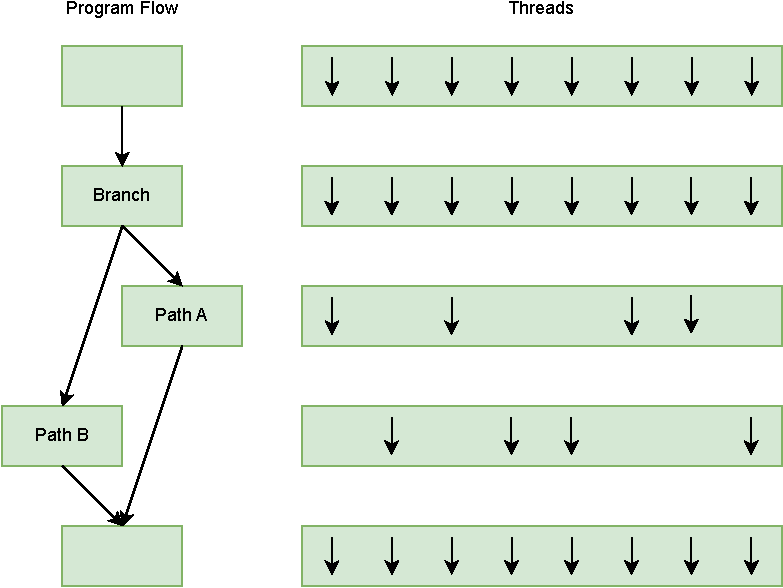
\includegraphics[width=0.65\textwidth]{Chapters/Figures/Images/control_div.pdf}
    \caption{Control flow divergence.}
\label{fig:control-div}
\end{figure}
    
    \paragraph{\textbf{Thread Cooperation}.} Threads within a block can cooperate via shared memory, atomic operations, and barrier synchronization. Each thread has its own local data, but threads within a block can use shared data. Data to be shared between threads can be declared using the \texttt{\_\_shared\_\_} keyword. There also exist primitives to perform block-wide barriers and atomic operations on data, however, these operations come at a performance cost, meaning that they should be used sparingly.
    
    \paragraph{\textbf{Overlapping Execution and Communication}.} The latency associated with transferring data between the host and device is very high. This means that the device cores can become idle for lots of clock cycles while communication with the host is being performed. In order to avoid this, it is possible to conduct communication asynchronously and bi-directionally while the device is performing computation. For example, considering a scenario where a lot of data has to be processed, it might be possible to partition the data into $N$ partitions, send the first partition to the device, and then while the second partition is being sent, the first partition can start being processed. \gls{CUDA} streams and events can be used for this purpose. Other usages of these mechanisms include asynchronous requests to the device to allow for concurrent execution between the host and device.

    \paragraph{\textbf{Global Memory Accesses}.}  Given that accesses to global memory are slow, it is important to make these accesses as efficient as possible. When fetching data, the bus can handle 128 bytes. The main caches are also divided into 128-byte cache lines. Accesses without caching are done via 32-byte segments (given that warps have 32 threads). To reduce the number of transactions required to fetch data, it is important to keep the memory accesses coalesced and aligned with the 128-byte cache lines and with the 32-byte segments. This way all the threads can fetch their respective data simultaneously.

    \paragraph{\textbf{Shared Memory Accesses}.} Within a \gls{SM}, threads can access a shared memory. This shared memory is divided into 32 banks which are 8 bytes (2 words) wide. If two (or more) different threads within a warp access the same bank, but do not access the same word, a bank conflict occurs 
    %(as exemplified in Figure~\ref{fig:bank-conflict})
    . Whenever there is a bank conflict, the accesses are performed sequentially. To avoid this, one should arrange the data accesses in such  a way that avoids these bank conflicts as much as possible. This can require using padding (sacrificing some shared memory space in favor of less latency) or remapping of the data. It should be noted that for devices of compute capability 2.0 and higher, the ability to multicast shared memory accesses has been added to mitigate this issue~\cite{blog:cuda_shared_memory}. This means that multiple accesses to the same location by any number of threads within a warp are served simultaneously.

% \begin{figure}
%   \centering
%     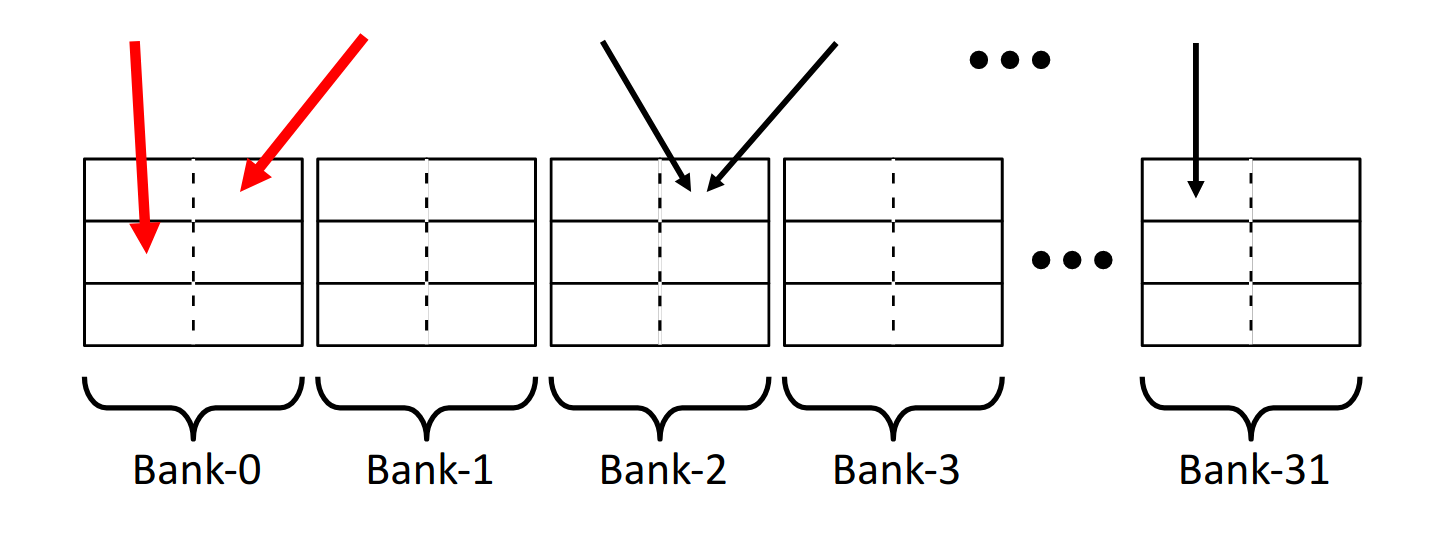
\includegraphics[width=0.75\textwidth]{Chapters/Figures/Images/bank_conflict.png}
%     \caption{Addresses from a warp: 2-way bank conflict}
% \label{fig:bank-conflict}
% \end{figure}


\section{Marrow}
\label{sec:marrow}

Marrow is a high-level C++ parallelization library that implements an algorithmic skeletons programming model. Skeletons comprise common algorithms such as map, scan, and reduce, which can be nested to express complex computations. Marrow parallelizes and executes these computations, and supports multiple backends to do so. It supports \gls{CUDA} and OpenCL backends for \gls{GPU} offloading, and an OpenMP backend for multi-threaded execution. Data in a marrow program can be represented using smart containers including vectors, arrays, scalars, matrices, and tensors. These containers offer a unified address space, meaning that the programmer does not need to worry about managing host and device memory (when dealing with \gls{GPU}-based backends). A data container can be seemingly accessed both on the host and the device. The programmer simply instantiates a set of containers, then applies skeletons and transformations over these containers, and marrow handles all the memory management and skeleton parallelization and execution.

\subsection{Using Marrow}

\begin{listing}
\begin{minted}
[
frame=lines,
linenos,
fontsize=\scriptsize
]
{cpp}
using T = float;
marrow::vector<T> x(100), y(100);
x.fill([] (int i){return rand();});
y.fill([] (int i){return rand();});

marrow::scalar<T> min = marrow::reduce<min<T>>(x);

auto sum = y + x;
marrow::vector<T> result_sum = min * sum;

auto dif = y - x;
marrow::vector<T> result_dif = min * dif;    
\end{minted}
\center
\caption{Marrow basic program.}
\label{lst:marrow}
\end{listing}

Listing~\ref{lst:marrow} shows a simple C++ program written using marrow. In lines 2-4, we create two vectors of equal size. In line 6, the min value from vector \texttt{x} is calculated using the \texttt{reduce} skeleton. In lines 8-9 the vectors are summed together (the \texttt{+} operator is equivalent to using the skeleton \texttt{map<plus>}) and then the result is multiplied by the previously computed scalar \texttt{min}. Lines 11-12 have a similar logic. As we can see, the programmer only specifies the containers and operations over these containers that he wishes to perform, and marrow converts these operations into kernels, launches them, and manages their execution and synchronization on the \gls{GPU} (assuming a backend such as \gls{CUDA} is used).  If a \gls{CUDA} backend is used, all skeletons are executed on the device. In this program, the vector \texttt{x} is initially allocated and filled on the host\footnote{Alternatively, we can configure marrow to perform this fill lazily on the device for better performance.} in line 3, then in line 6, the vector \texttt{x} is transferred to the device and the \texttt{min} scalar is computed by a kernel on the device as well.

Commonly used functions like map, reduce, scan and filter are provided by marrow, and can be applied to the various containers. Marrow also provides common operators such as min, max, plus, minus, multiplies, etc to use alongside the skeletons (for example \texttt{reduce<max>} or \texttt{map<plus>}). Alternatively, the programmer can define his own functors and pass them to the skeletons. Operator overloading is also provided for common map operations such as arithmetic functions between the different container types. In listing~\ref{lst:marrow} we can see that to perform arithmetic operations between vectors, instead of using a map skeleton with the corresponding arithmetic operator, the programmer can simply use the overloaded functions plus, minus, multiplication, etc.

Marrow also supports custom functions to process and generate containers. These are denominated \texttt{marrow::function} and operate as a more generic map operator. Marrow functions can take as arguments any number of marrow containers of any size, any number of primitive data types, and return a single marrow container. These functions can also receive coordinates as a parameter, which is useful when dealing with backends such as \gls{CUDA}. Moreover, the parameters of a marrow function can optionally be marked as \texttt{in}, \texttt{out}, or \texttt{inout}, to specify if a parameter is intended as an input, an output container, or both. The geometry of the function, i.e. the grid geometry in the case of a backend such as \gls{CUDA}, is implicitly calculated by marrow, but can also be set by the programmer. 

Listing~\ref{lst:marrow_mandelbrot_fun} illustrates a marrow function \texttt{mandelbrot\_fun} that can take as input a \texttt{vector<int>} and an integer \texttt{n}, and outputs a \texttt{vector<int>} representing the pixel values of a discrete mandelbrot set. In lines 1-2 we define an auxiliary function \texttt{divergence} annotated with \texttt{marrow\_function}. This annotation is necessary for dealing with backends such as \gls{CUDA} that require decorators such as \texttt{\_\_device\_\_}. In lines 4-14 we define a functor \texttt{mandelbrot\_fun} that extends \texttt{marrow::function} passing as template parameters the functor itself, the return type, and the types of the arguments. In the body of the function we describe the logic we wish to perform on each element \texttt{pos} of the input container. In lines 17-22 we define a C++ function that starts by generating a vector \texttt{positions} of size $n*n$ of counting integers \footnote{Not actually a vector but rather an expression that evaluates to such a vector.}, then instantiates a \texttt{mandelbrot\_fun} object, and finally applies \texttt{positions} and \texttt{n} to the marrow function and stores the result in the marrow vector \texttt{x}. Note that this specific example could also be written using a map skeleton with a similar functor instead.

% mandelbrot example


\begin{listing}
\begin{minted}
[
frame=lines,
linenos,
fontsize=\scriptsize
]
{cpp}
marrow_function 
int divergence(int depth, marrow::complex<float> c0) { ... }

struct mandelbrot_fun : public marrow::function<mandelbrot_fun, int, int, int> {

    marrow_function
    int operator()(int pos, int n) {

        int x = pos / n;
        int y = pos % n;
        marrow::complex<float> c0(XMIN + x * SIZEX / n, YMIN + y * SIZEY / n);
        return divergence(DEPTH, c0);
    }
};

marrow::vector<int> mandelbrot(int n) {
    mandelbrot_fun mandelbrot_f;
    auto positions = iota(n*n); // expression that evalutes to a marrow::vector<int>
    marrow::vector<int> x = mandelbrot_f(positions, n);
    return x;
}  
\end{minted}
\center
\caption{Marrow mandelbrot function.}
\label{lst:marrow_mandelbrot_fun}
\end{listing}


Listing~\ref{lst:marrow_foo_fun} illustrates a more complex marrow function \texttt{foo\_fun}. In line 21 we pass a container of integers, a container of floats, and a single integer \texttt{n} to \texttt{foo\_f}. However, the functor receives as parameters an integer, a collection of floats (float pointer), and another integer (besides the function coordinates \texttt{c}). This implicitly states that the function will operate in parallel over the elements of \texttt{indexes} while delegating accesses to the container \texttt{values} to the programmer. In this case, we access the elements of \texttt{values} using the function coordinates. By providing the correct data types in the function's template parameters, Marrow is able to handle this distinction. Finally, the function will return a container of the same size as \texttt{indexes}, but of type float.


\begin{listing}
\begin{minted}
[
frame=lines,
linenos,
fontsize=\scriptsize
]
{cpp}
marrow_function 
float bar(float x, float y) { ... }

struct foo_fun : public marrow::function_with_coordinates<foo_fun, float, int, float*, int> {

    marrow_function
    float operator()(coordinates_t c, int index, float* values, int n) {

        int coordinate_index = c[0] % n;
        return bar(values[index], values[coordinate_index]);
    }
};


marrow::vector<float> foo(int n) {
    
    foo_fun foo_f;
    marrow::vector<int> values = ...;
    marrow::vector<float> indexes = ...;
    // set values of indexes and values
    marrow::vector<float> result = foo_f(indexes, values, n);
    return x;
}
\end{minted}
\center
\caption{Marrow foo function.}
\label{lst:marrow_foo_fun}
\end{listing}

You may notice that in listings~\ref{lst:marrow} and~\ref{lst:marrow_mandelbrot_fun} we sometimes use the \texttt{auto} keyword when defining the variables that receive the result of a given operation over containers. The reason is that whenever we apply a skeleton or function over a set of containers, instead of triggering the corresponding computation, we are simply defining a template expression that describes the desired computation. Only when such an expression is assigned to a container is the expression actually evaluated and therefore computed. This means that in line 8 of listing~\ref{lst:marrow}, no computation is launched, and the type of \texttt{sum} isn't a container, but rather a marrow expression. Only in line 9, where the result of the expression \texttt{min * sum} is assigned to the vector \texttt{result\_sum}, is the expression actually evaluated. This allows marrow to compute the vector \texttt{result\_sum} in a single kernel (more on this later). As a rule of thumb, whenever the result of a computation is explicitly required or is used in multiple succeeding computations, we assign it to a corresponding container, otherwise, the \texttt{auto} keyword can be used to simply obtain the desired marrow expression. 

\subsection{Marrow Architecture}

Marrow is comprised of 3 layers (as seen in Figure~\ref{fig:marro_architecture}): API, runtime, and backends. The user only interfaces with the upper layer. This layer includes all the supported containers, functions, operators, and skeletons. During compilation, kernels are generated from the computations the user-defined, using the marrow API, for a specified backend such as \gls{CUDA}. Its then the job of the runtime layer to launch and manage these kernels, as well as ensuring any necessary data synchronization. To this end, the runtime 
is composed of a scheduler, a dependency manager and a task manager. These components utilizes generic modules such as marrow events and marrow allocators, which in turn delegate backend-specific calls to the backend layer.

\begin{figure}[tbp]
  \centering
    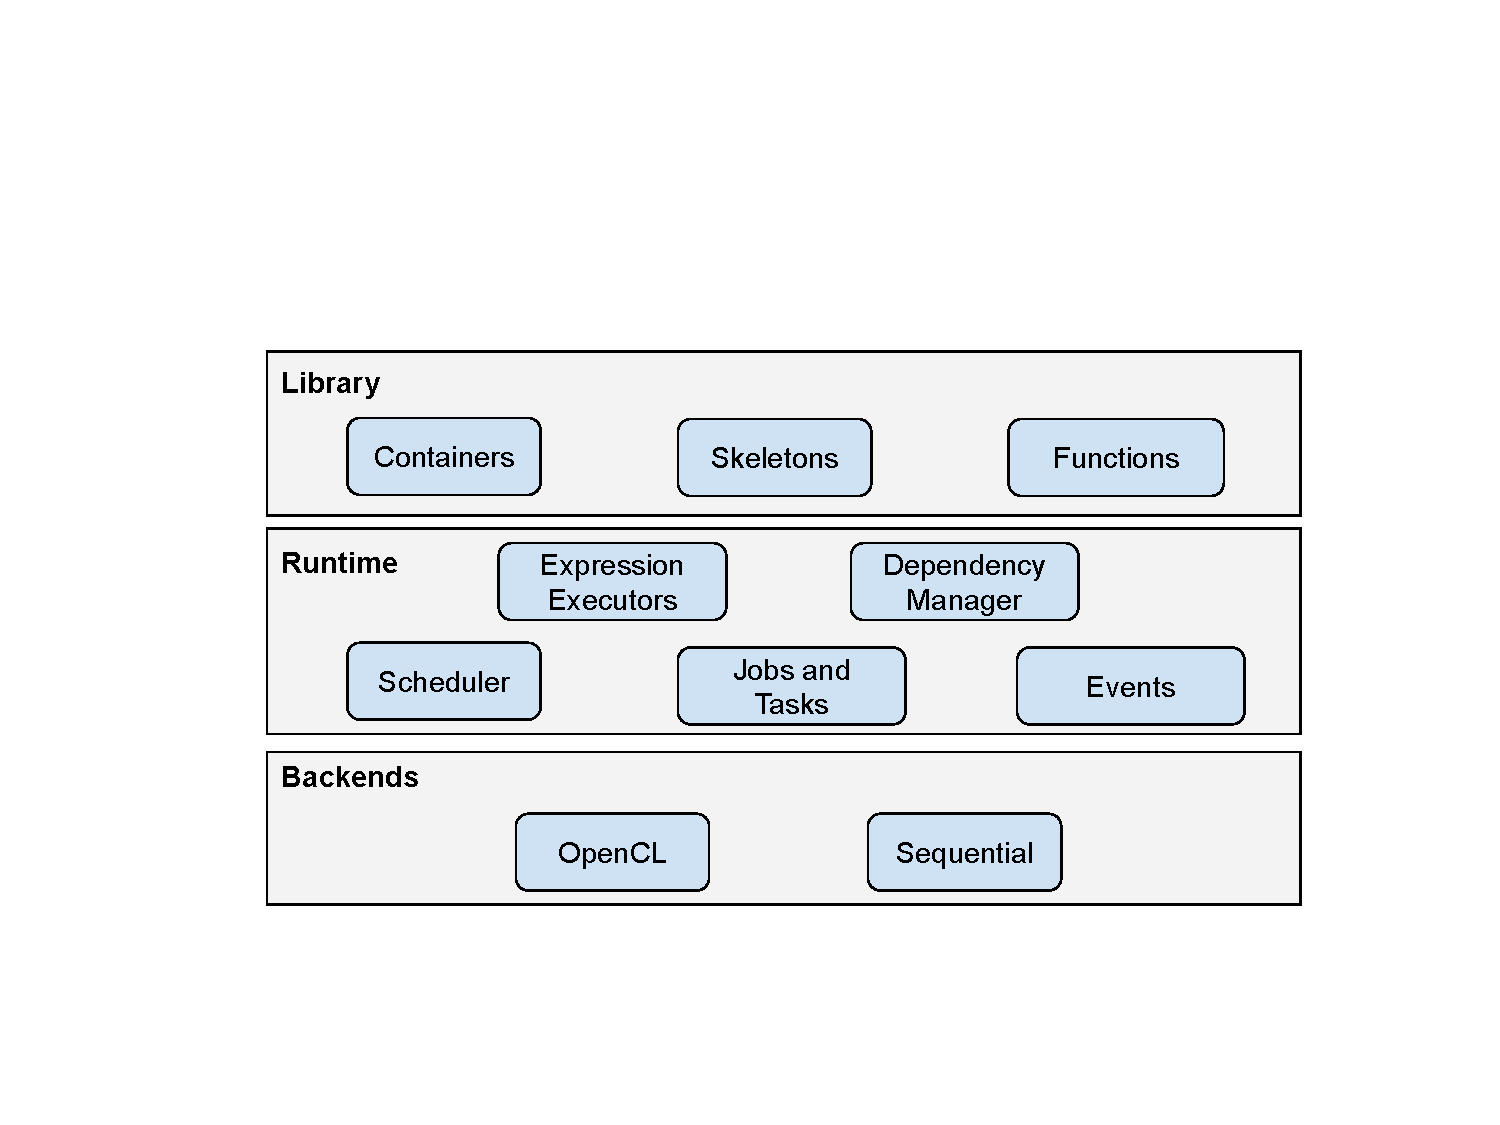
\includegraphics[width=0.7\textwidth]{Chapters/Figures/Images/marrow_architecture.pdf}
    \caption{Marrow architecture.}
\label{fig:marro_architecture}
\end{figure}

% The backend layer therefore includes all the backend specific code necessary for generating, launching, managing and communicating with the kernels. It also handles events and any necessary memory allocation and transfers.
% The runtime then launches and manages those kernels. The runtime includes a scheduler, dependency manager and a task manager.

As previously mentioned, to avoid generating a separate kernel for each operation/function, marrow expressions are subjected to lazy evaluation. This ensures that a marrow expression's result is only computed when it is required or specifically requested. To this end, marrow makes use of \gls{AST}s which can include multiple operations/functions. Potentially a single kernel is generated for an entire \gls{AST}. Returning to Listing~\ref{lst:marrow}, in lines 8 and 11, the \texttt{auto} keyword is used to define the type of the variables \texttt{sum} and \texttt{dif}, meaning that these variables store marrow expressions. In line 9 we have another variable assignment, but this time, the type of the variable is a marrow container. This informs marrow that the expression on the right-hand side of the expression should be evaluated, and its result stored in the variable \texttt{result\_sum}. The \gls{AST} that is computed in this line is represented in Figure~\ref{fig:ast} (as well as the \gls{AST}s that are computed in lines 6 and 12 respectively). We can see that the \gls{AST} includes both the sum between \texttt{x} and \texttt{y}, and the multiplication of \texttt{min} with the previous result. This optimization can drastically decrease the communication and memory transferred between the host and device. Note that sometimes it is not desired to use the \texttt{auto} keyword if a variable is later used multiple times, like variable \texttt{min} in line 6 for example, since this will result in the value being computed multiple times in different kernels.

\begin{figure}[tbp]
  \centering
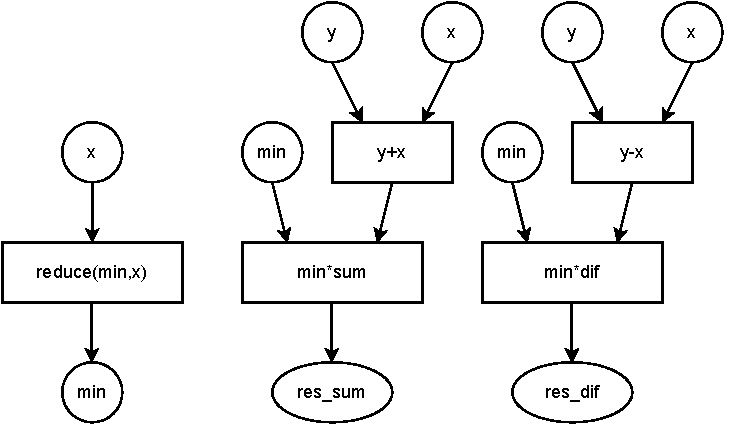
\includegraphics[width=0.8\textwidth]{Chapters/Figures/Images/ast.pdf}
    \caption{Marrow program \gls{AST}s.}
\label{fig:ast}
\end{figure}

Another optimization implemented by marrow is the usage of non-blocking kernel execution. Whenever a computation is launched, like in lines 6, 9, and 12 from listing~\ref{lst:marrow}, the program follows to the next instruction without blocking until the computation is over. Of course, if the result of a computation is required in another line of the program, the program waits for the result to be computed before proceeding. All this logic is handled by the runtime dependency manager and scheduler.




% intro



\begin{figure}[tbp]
  \centering
    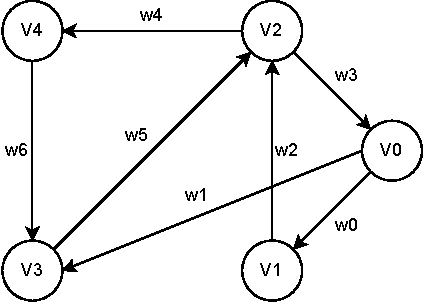
\includegraphics[width=0.5\textwidth]{Chapters/Figures/Images/graph_a.pdf}
    \caption{Directed graph.}
    \label{fig:graph-a}
\end{figure}

    \section{Graph Data Structures} \label{graph_data_structures}
    \label{sec:graph_data_structures}
    
    We will now present the different data structures that can be used to represent graphs and discuss which are better suited for our purpose. This is not an exhaustive list of all the specific data structures used by the various graph processing frameworks, but rather a high-level view of the most common structures to represent graphs. Since our goal is to develop a \gls{GPU}-based dynamic graph library, these three characteristics should be taken into account:
    
    \begin{enumerate}
        \item \textbf{Random access speed:} Fast random accesses allow for fast algorithms to be performed over the graph and help us leverage parallelism. 
        \item \textbf{Compactness:} A compact representation of the graph allows us to take as much advantage of the limited \gls{GPU} memory as possible, and to reduce the amount of data transfers between the host and device.
        \item \textbf{Update-friendliness:} A dynamic graph data structure must allow for efficient updates to the graph.
    \end{enumerate}

    The most common data structures used to represent graphs are the following:

    \paragraph{\textbf{Adjacency Matrix}.} Storing a graph in an adjacency matrix is straightforward. Each cell $C_{i,j}$ (row $i$, column $j$), stores the weight of the edge that goes from vertex $V_i$ to vertex $V_j$, if the edge exists. This representation allows for simple memory allocation strategies and fast random accesses. However, for sparse graphs\footnote{A graph in which most pairs of vertices are not connected by edges.}, this leads to a lot of wasted memory and sparse data, as can be seen in the adjacency matrix in Figure~\ref{fig:graph-a-matrix} (opposed to contiguous data, which usually allows for better performance).


\begin{figure}[tbp]
  \centering
    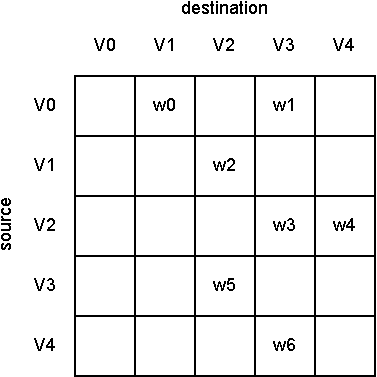
\includegraphics[width=0.4\textwidth]{Chapters/Figures/Images/graph_a_matrix.pdf}
    \caption{Adjacency matrix representation of graph~\ref{fig:graph-a}.}
\label{fig:graph-a-matrix}
\end{figure}

    \paragraph{\textbf{Adjacency List}.} An adjacency list represents a graph as an array of lists. For each vertex $V_i$, we define a list of adjacencies with all the vertices $V_j$, for which there exists an edge from $V_i$ to $V_j$. This way, no memory is wasted for non-existing edges, contrary to an adjacency matrix. The main issue with this approach is related with the way these lists are stored. The different lists will most likely not be stored contiguously. Moreover, some list implementations, like linked lists, do not store the the elements of a list contiguously. This kind of memory layout usually does not perform well in high-performance and parallel environments. Edge searches are also slower compared to an adjacency matrix given that the neighbors of the source index must be traversed to search for a specific edge. An example of an adjacency list can be seen in Figure~\ref{fig:graph-a-list}.

    In order to improve data locality, some graph representations use blocked adjacency lists~\cite{paper:faimgraph, paper:stinger}. In blocked adjacency lists, neighboring vertices of a given vertex $v$ are stored in fixed-sized blocks. For adjacency lists composed of multiple blocks, each block points to the next one. A small block size results in the same restrictions of a linked list whilst a large edge block has similar drawbacks of an adjacency matrix. This strategy allows one to trade some memory overhead for better locality. 

\begin{figure}[tbp]
  \centering
    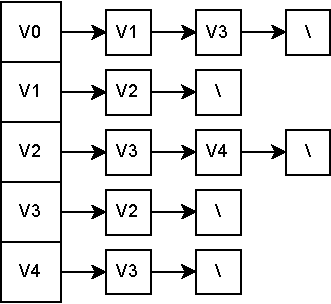
\includegraphics[width=0.4\textwidth]{Chapters/Figures/Images/graph_a_list.pdf}
    \caption{Adjacency list representation of graph~\ref{fig:graph-a}.}
\label{fig:graph-a-list}
\end{figure}

    \paragraph{\textbf{Compact Sparse Rows}.} \gls{CSR} is considered to be the most compact data structure to store graphs. This data structure consists of 3 arrays (or vectors) as seen in Figure~\ref{fig:graph-a-csr}. The two ``parallel'' arrays, \texttt{col\_indexes} and \texttt{values}, store the information about the edges and have a length equal to the number of edges in the graph. The array \texttt{row\_offsets}, has a length equal to the number of vertices in the graph. Each element $O_i$ of the array \texttt{row\_offsets}, stores the offset where the information, about the outgoing edges from vertex $V_i$, starts. \texttt{col\_indexes} stores the indexes (or IDs) of the destination vertices of the edges, and the array \texttt{values} stores the corresponding weights. Given that all the outgoing edges from a given vertex $V_i$ are stored contiguously, the degree of $V_i$ can be calculated using the offsets array as follows: \texttt{row\_offsets[i+1] - row\_offsets[i]}. Even though \gls{CSR} features good compactness and locality, updating a graph represented using \gls{CSR}, requires reconstructing the whole data structure.

    In order to address the last issue, some bodies of work~\cite{paper:pcsr, paper:csrpp} have proposed modifications to \gls{CSR}, in order to support relatively efficient manipulations to the graph. CSR++~\cite{paper:csrpp} uses a segmentation technique, keeping vertices and neighbor edges compacted. It stores vertices in segments, where each segment is a fixed-size array. Edges are stored using per-vertex arrays. Vertex property values are stored in parallel arrays within each segment. For edge properties, a similar segmentation approach is used. Each vertex structure stores a pointer to an array of edge property values. The property values can be located using offsets and calculations based on the type, index, and degree of the vertex. \gls{PCSR}~\cite{paper:pcsr} bases its implementation on a dynamic array-based data structure called \gls{PMA}. \gls{PCSR} is similar to \gls{CSR}, but leaves space between elements, allowing for significantly faster insertions and deletions while slowing traversal times by a constant factor. As far as we know, none of these \gls{CSR} adaptations have been implemented in GPU environments.

\begin{figure}[tbp]
  \centering
    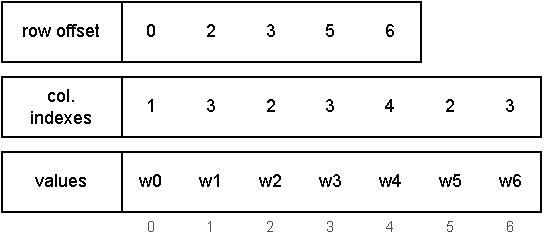
\includegraphics[width=0.6\textwidth]{Chapters/Figures/Images/graph_a_csr.pdf}
    \caption{\gls{CSR} representation of graph~\ref{fig:graph-a}.}
\label{fig:graph-a-csr}
\end{figure}

    \paragraph{\textbf{Vector Graph}~\cite{vgraph}.} Vector graph stores a graph using a segmented vector. Each segment corresponds to a vertex, and the number of elements in a given segment corresponds to the degree of the associated vertex. The values kept in the elements of the segmented vector are pointers to the other end of the edge. More vectors can be added to store information about weights, vertex IDs, etc. Figure~\ref{fig:graph-a-vgraph} shows an example of a vector graph representation. Vector \texttt{vertex} stores the ID of the vertex of each segment. Vector \texttt{segment-descriptor} stores the degree of the vertices of each segment. Vectors \texttt{cross-pointer} and \texttt{weights} store the pointers to the other end of the edges and the weights associated with each edge. For undirected graphs, this representation results in duplicated information. Like \gls{CSR}, updating a graph requires reconstructing the whole data structure. %It does however, allow for fast random accesses given that all the edges are stored contiguously.
    

\begin{figure}[tbp]
  \centering
    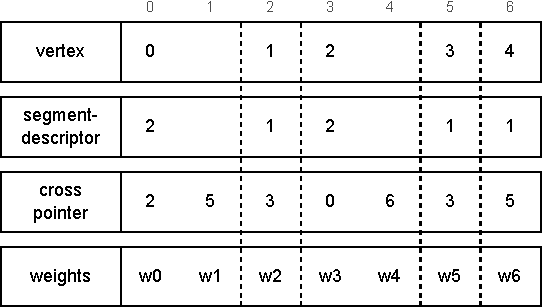
\includegraphics[width=0.6\textwidth]{Chapters/Figures/Images/graph_a_vgraph.pdf}
    \caption{Vector graph representation of graph~\ref{fig:graph-a}.}
\label{fig:graph-a-vgraph}
\end{figure}

    % \paragraph{\textbf{STINGER}~\cite{paper:stinger}.} \gls{STINGER} uses features from \gls{CSR}, adjacency lists and adjacency matrices, allowing for fast updates. The data structure is based on linked-lists of blocks. Each block stores multiple edges and is referred to as an edge block. It is possible to grow the graph by adding new edge blocks. The edge block size is a user controlled parameter. A small edge block size results in the same restrictions of a linked list whilst a large edge block has the same drawbacks of an adjacency matrix. Therefore this parameter should be selected based on the characteristics of the graph that will be processed.
    % TODO: limitations

    % data-structure that represents a graph as a set of pages
    % each page is stored in a contiguous area of memory
    % a page is divided in two logical areas. An area of slots, which typically starts at the end of the page and grows towards the beginning of the page, and an area of records,which typically starts at the start of the page and grows towards the end of the page. 
    % The slots store the adjacency lists of the vertices stored in the page. 
    % The records store information that allows one to get the location of an adjacency list for a given vertex ID.
    % Some implementations of slotted pages also include metadata at the start of the slotted page.
    % All slotted pages have a fixed size. Vertices and edges can be added to a slotted page until it’s full, at which point, a new slotted page is created.
    % If an adjacency list of a vertex doesn’t fit in a single slotted page, extra Large Adjancey Pages are created.
    % Allows for regular accesses
    % is semi-compact
    % allows for efficient updates

    \paragraph{\textbf{Slotted Pages}~\cite{paper:turbograph}.} Slotted pages is a data structure that represents a graph as a set of pages. Each page is stored in a contiguous area of memory. A page is divided into two logical areas. An area of slots, which typically starts at the end of the page and grows towards the beginning of the page, and an area of records, which typically starts at the start of the page and grows towards the end of the page. The slots store the adjacency lists of the vertices stored in the page. The records store information that allows one to get the location of an adjacency list for a given vertex ID. Some implementations of slotted pages also include metadata at the start of the slotted page, like the number of vertices stored on the page. All slotted pages have the same fixed size. Vertices and edges can be added to a slotted page until it is full, at which point, a new slotted page is created. If an adjacency list of a vertex does not fit in a single slotted page, extra Large Adjacency Pages are created. This data structure is an appealing data structure for dynamic graphs, and has been used by dynamic graph processing frameworks like TurboGraph~\cite{paper:turbograph}, since it allows for regular accesses, is semi-compact, and allows for efficient updates.

    \subsubsection*{\textbf{Conclusions}}

    From Table~\ref{tab:graph_data_structures} we derive a comparison between the previously presented data structures. \gls{CSR} and vector graph offer the best compactness and memory locality but are subjected to extremely slow updates. However, \gls{CSR} variants that trade some compactness and locality for faster updates can be a viable option for representing a dynamic graph on a \gls{GPU}. Adjacency Matrices, even though offer the fastest edge searches, have the worst spacial complexity and are generally too sparse considering the limitations of \gls{GPU} memory (this doesn't apply when considering dense graphs, however, a lot of large-scale real-life graphs are sparse). Adjacency lists offer good characteristics overall, but as discussed before, their memory layout isn't well suited for \gls{GPU}s. Blocked adjacency lists and slotted pages offer a good balance between compactness, memory locality, and update efficiency. In both cases, compactness and locality are proportional to the size of the blocks or pages. Blocked adjacency lists offer some faster updates and search operations compared to slotted pages. This is due to the overheads associated with searching for a page that contains a given vertex, and the in-page reallocations. Slotted pages can however offer better memory locality for sparse graphs, given that a single page can store multiple adjacency lists.

% complexidade espacial 
% complexidade temporal das ops
% insert/remove -- traversal
% dinamica?
% direccionado / pesos
% GPU (existe ou se é intuitavemente eficientemente implementável)

    % PCSR ?
    % Hash-Table based ?
    % \gls{CSR}++ ?
    % Segmented \gls{CSR} ?


    % conclusions

    % 

    \begin{table}[tbp]
        \scriptsize
        \centering
        \begin{tabular}{| c | c c c c c |}
            \hline
              & \makecell{Adjacency \\ Matrix} & \makecell{Adjacency \\ List} & \makecell{Blocked \\ Adjacency List} & CSR & \makecell{Slotted \\ Pages} \\
            \hline
            \hline
            Dynamic & yes & yes & yes & no & yes \\
            %\hline
            Directed & yes & yes & yes & yes & yes \\
            %\hline
            Mem. Locality & poor & poor & $\propto s_b$ & optimal & $\propto s_p$ \\
            %\hline
            Spacial Cost & $O(n^2)$ & $O(n+m)$ & $O(n+(1+f_b)*m)$ & $O(n+m)$ & $O(n+(1+f_p)*m)$ \\
            Search Edge $(v_1,v_2)$ & $O(1)$ & $O(deg(v_1))$ & $O(deg(v_1))$ & $O(deg(v_1))$ & $O(log(n_p) + deg(v_1))$ \\ 
            Add Vertex & $O(n^2)$ & $O(1)$ & $O(1)$ & $O(n+m)$\* & $O(1)$ \\ 
            Del Vertex $v$ & $O(n^2)$ & $O(deg(v))$ & $O(deg(v))$ & $O(n+m)$ & $O(log(n_p) + s_p)$ \\
            Add Edge & $O(1)$ & $O(1)$ & $O(1)$ & $O(n+m)$ & $O(log(n_p) + s_p)$ \\
            Del Edge $(v_1, v_2)$ & $O(1)$ & $O(deg(v_1))$ & $O(deg(v_1))$ & $O(n+m)$ & $O(log(n_p) + deg(v_1) + s_p)$ \\
            %\hline
            
            \hline
        \end{tabular}
        \caption{Graph data structure comparison with an approximation of each one's spacial complexity and temporal complexity for a set of operations. Note that for vertex deletion complexity, we are ignoring possible necessary destination vertex deletions ($n = |\text{vertices}|$, $m = |\text{Edges}|$, $s_b = \text{block size}$, $s_p = \text{page size}$, $n_p = \text{number of pages}$, $f_b \propto S_b = \text{blocked adjacency list fragmentation proportion}$, $f_p \propto S_p = \text{slotted pages fragmentation proportion}$).}
        \label{tab:graph_data_structures}.
    \end{table}
    
    \section{Graph Programming Models}
    \label{sec:programming_models}

    In order to process graphs, one can consider different units of parallel execution and different programming models. In this section, we introduce some of the most common units and models, and in the following section, we discuss how these are implemented by some of the existing graph processing frameworks. 
    % The three main units are:

    \subsection{Units}

    \paragraph{\textbf{Vertex-Centric}.} In vertex-centric programming models, the processing algorithms are expressed from the perspective of a vertex. This means that the user defines a vertex-local function
    %, which receives information from the neighboring vertices, performs a computation, possibly updates the vertex, and sends information to the outgoing edges. 
    , which can receive and send information from/to its neighboring vertices. 
    The vertex therefore becomes the unit for parallel execution. This concept was formally introduced by Pregel~\cite{paper:pregel} and later used by other frameworks like GraphLab~\cite{paper:graphlab} and PowerGraph~\cite{paper:powergraph}.

    \paragraph{\textbf{Edge-Centric}.} In edge-centric programming models, the processing algorithms are expressed from the perspective of an edge. This paradigm was adopted by systems like X-Stream~\cite{paper:xstream} and Chaos~\cite{paper:chaos}. This unit can potentially ease load balancing given that it does not deal with variable vertex degrees like the vertex-centric unit. 
    %for optimizing the usage of secondary storage and network communication with cloud-based machines to process large graphs.
 
    \paragraph{\textbf{Sub-Graph-Centric}.} Both vertex-centric and edge-centric models are fine-grained, given that the unit of parallel execution is the vertex and the edge respectively. This can lead to large communication overheads in distributed systems. Sub-graph-centric models therefore aim to reduce these overheads by using a sub-graph structure as the unit of parallel execution (coarse-grained). Two approaches are used for this end, partition-centric and neighbourhood-centric. The first partitions the graph into multiple sub-graphs which can be processed in parallel. Each vertex can send information to any other vertex within the same partition, opposed to a vertex-centric approach, where a vertex can only send information to its neighboring vertices. This paradigm has been adopted by Giraph++ for example. Neighbourhood-centric models on the other hand, allow for multiple sub-graphs to exist within a physical partition. This paradigm facilitates the implementation of graph algorithms that operate on ego networks; networks built around a central vertex of interest. In such algorithms, the user might want to define a set of custom sub-graphs which are built around vertices and their multi-hop neighbors. Shared-state updates are used to exchange information between sub-graphs in the same partition, and replicas and messages are used to exchange information between sub-graphs in different partitions~\cite{paper:high_level_distributed_graph}.
    

    % The most common programming models are:
    \subsection{Models}

    %\paragraph{\textbf{Superstep}.} A user-defined function is executed on all vertices in parallel. Once the function has finished executing on all vertices, messages can be exchanged between the vertices and processed by a user-defined function.

    \paragraph{\textbf{Bulk Synchronous}.} Bulk synchronous executes an algorithm in supersteps. A superstep consists of a sequence of three steps (as shown in Figure~\ref{fig:bsp}):
    \begin{enumerate}
        \item \textbf{Concurrent Computation:} Each processor performs a local computation.
        \item \textbf{Communication:} Processors exchange data.
        \item \textbf{Barrier Synchronization:} Synchronizes all processors.
    \end{enumerate}
    %
    In graph processing, during each superstep, a user-defined function is applied to all the vertices asynchronously. The results are then sent to each vertice's neighbors. 
    %When implementing this model using \gls{GPU}s, the graph is usually partitioned in $N$ sectors and a kernel is launched for each sector during a supertep. During the concurrent computation step, all kernel execute simultaneously, and all threads execute concurrently. During the communication step, threads within a kernel communicate using local memory, and if needed, kernels can send messages to their neighours. In the end of the superstep, all the kernels are synchronized. 
    When implementing this model using \gls{GPU}s, a superstep is performed by one or more kernels. Threads within a kernel execute concurrently. Communication between threads is performed via local-memory and communication between supersteps via global-memory. Synchronization between supersteps is achieved by a barrier that waits for the kernel (or multiple kernels) to finish before continuing.
    This model has been adopted by frameworks like Pregel~\cite{paper:pregel}, Gunrock~\cite{paper:gunrock} and Medusa~\cite{paper:medusa}, and is the best suited for \gls{GPU} acceleration, given that a superstep can simply be modeled with a kernel launch.

\begin{figure}[tbp]
  \centering
    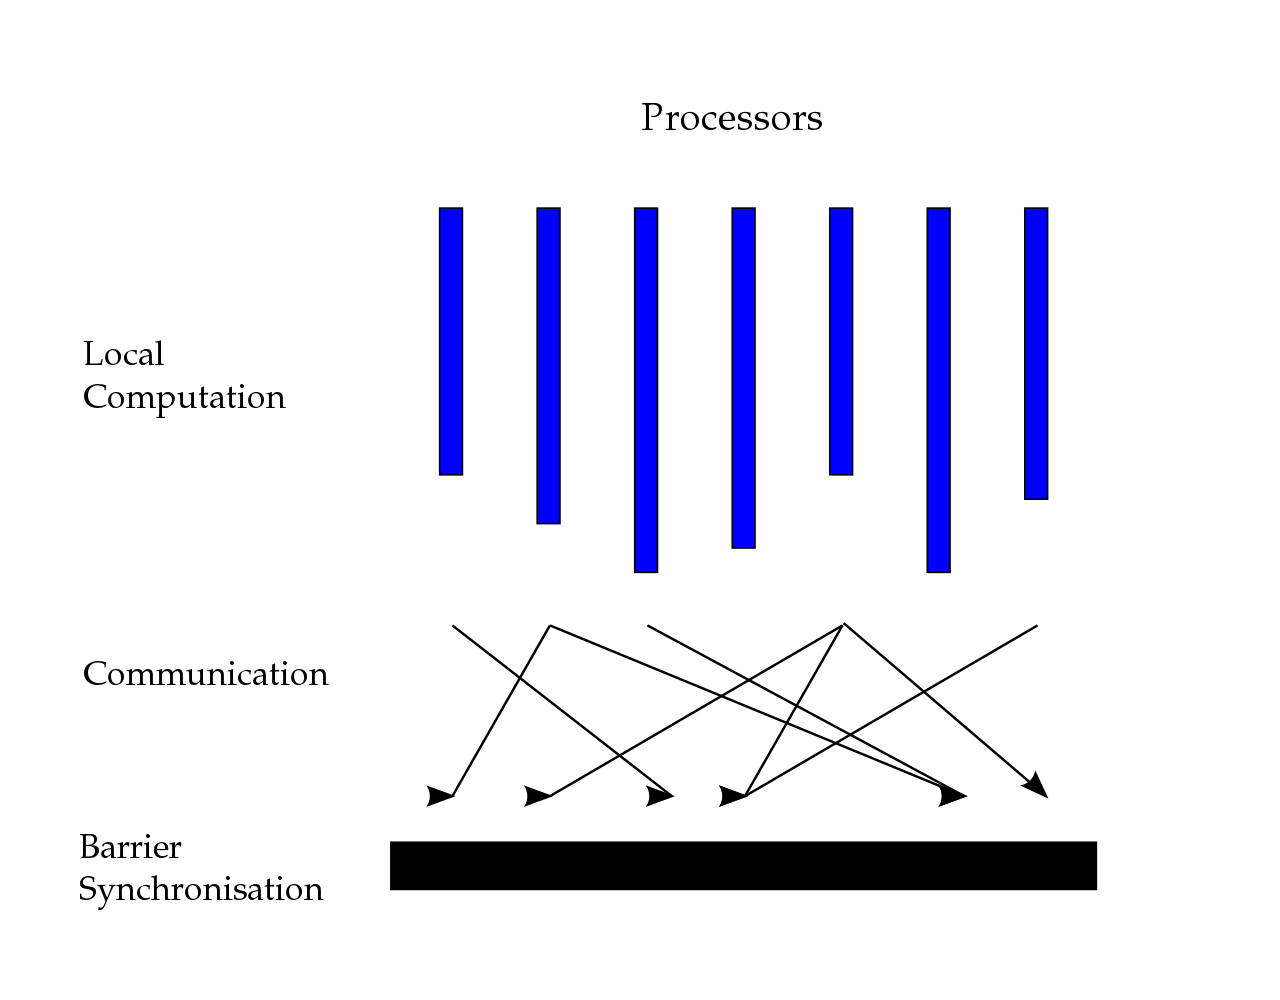
\includegraphics[width=0.75\textwidth]{Chapters/Figures/Images/bsp.png}
    \caption{Bulk synchronous parallel superstep (taken from~\cite{wiki:bsp}).}
\label{fig:bsp}
\end{figure}

    \paragraph{\textbf{Scatter-Gather}.} This model consists of two phases, each dictated by a user-defined function. In the scatter phase, each vertex sends messages to its neighbors. In the gather phase, each vertex receives messages from its neighbors and performs a computation, possibly updating its state.
    
    \paragraph{\textbf{Gather‑Apply‑Scatter}.} This model was introduced by PowerGraph~\cite{paper:powergraph} to solve issues present with other models regarding power-law graphs, given that big differences between the degrees of vertices could lead to computational load imbalances (vertices with high degrees become stragglers). To solve this, the vertex-local function/program is decomposed into multiple phases, which can be more evenly distributed across a cluster. It consists of three phases, each dictated by a user-defined function and executed in parallel.  In the gather phase, each vertex receives information from its neighboring vertices. In the apply phase, each vertex performs a computation and possibly updates its state. In the scatter phase, each vertex sends information regarding its new state to its outgoing edges. Some algorithms do not require the gather phase.
    
    \section{Graph Processing}

    In this section we will present some of the existing state-of-the-art high-performance graph processing frameworks, discussing their key features, data models, and programming models. All the frameworks that were analysed can be found in table~\ref{tab:graph_processing_frameworks}, however, in this section, we will only address the ones we found to be the most relevant for our purpose. Given our goal, we will give a more detailed analysis of the \gls{GPU} based solutions.

    
    \subsection{Distributed}
    
    %\paragraph{\textbf{Distributed}.} 
    As we can see in Figure~\ref{tab:graph_processing_frameworks}, most distributed graph frameworks, i.e. intended for clusters, are vertex-centric, with some exceptions, and represent their graphs using data structures which can easily be partitioned, like edge lists and adjacency lists.

    % ref: survey
    % PBGL (which is an extension of Boost’s graph library) stores its graphs as distributed adjacency lists where each compute resource is given ownership of a vertex and its outgoing edges. It also makes use of a generic programming paradigmn to provide a library that allows distributed computation on graphs~\cite{survey:graph_processing_landscape}.

    % ref: survey
    % CombBLAS has a different approach to graph processing, using sparse arrays to offer linear algebra primitives. It uses a sparse matrix data structure to represent the graph's adjacency matrix, and is edge-centric given that the elements of the matrix, on which the computations are performed, represent the edges of the graph~\cite{survey:graph_processing_landscape}.
    % It also decouples the parallel logic from the sequential parts of the computation.

    \paragraph{\textbf{GraphIn}.} 
    % ref: https://www.researchgate.net/publication/303786170_GraphIn_An_Online_High_Performance_Incremental_Graph_Processing_Framework
    GraphIn~\cite{paper:graphin} adopts a hybrid data structure using a compressed matrix format to store a static version of the graph and edge lists to store updates. The edge list allows for fast updates, while the compressed format allows for fast parallel computation. GraphIn merges these two data structures whenever it is required.

    \paragraph{\textbf{Chaos}.} 
    % ref: survey
    Chaos~\cite{paper:chaos} has its foundations on X-Stream~\cite{paper:xstream}, using sequential storage accesses and an adaptation of X-Stream’s streaming partitions which allow for parallel execution. Its design ensures that the storage devices are busy as much as possible in order to optimize for the bandwidth bottleneck. Both Chaos and XStream are novel in using an edge-centric (instead of vertex-centric) implementation of the scatter-gather model, and for streaming unordered edge lists instead of utilizing random accesses which are slower when using storage devices~\cite{survey:graph_processing_landscape}.

    \paragraph{\textbf{PowerGraph}.} 
    % ref: https://www.usenix.org/conference/osdi12/technical-sessions/presentation/gonzalez
    PowerGraph~\cite{paper:powergraph} is an extension of GraphLab, and offers a different approach to representing distributed graphs by exploiting the structure of power-law graphs. It presents e graph-parallel abstraction based on \gls{GAS}, which eliminates the degree dependence found in vertex-centric programs. It does so by leveraging the \gls{GAS} decomposition, factoring the vertex programs over edges. This way, PowerGraph maintains the "think-like-a-vertex" paradigm but is able to distribute the computation of a single vertex over a cluster.

    \paragraph{\textbf{GraphX}.} 
    % ref: https://www.usenix.org/conference/osdi14/technical-sessions/presentation/gonzalez
    Most of the frameworks so far are specialized graph processing systems. GraphX~\cite{paper:graphx} on the other hand, is built on top of Spark, a general-purpose distributed dataflow framework. It presents a common graph API, which is implemented using a few basic dataflow operators, like join, map, group-by, etc. To achieve a good performance, graph-specific optimizations are implemented using distributed join optimizations and other distributed techniques.
    %materialized view maintenance. 
    Internally the graphs are stored using a pair of vertex and edge collections built on the Spark RDD.

    \paragraph{\textbf{Pregel}.} 
    Google's Pregel library divides a graph into partitions, each consisting of a set of vertices and all of those vertices’ outgoing edges. Its main contribution is the introduction of a simple vertex-centric API that automatically scales efficiently.

    \subsection{CPU-Based}

    Shared memory multi-core \gls{CPU} machines have the advantage of not having to deal with communication overheads and data partitioning, however, they also have limited potential for parallelization. Given that modern \gls{CPU}s can perform complex operations very fast, frameworks on these machines can take advantage of more complex data structures, like hash-tables~\cite{paper:ringo}, snapshot-based data structures~\cite{paper:llama} and even NUMA-Aware data layouts~\cite{paper:polymer}, which can be harder to implement efficiently in distributed or \gls{GPU}-based environments. We will now discuss three cases of study, chosen for their novel data structures and/or simplicity.
    %Most of the single machine frameworks that we found were vertex-centric.

    \paragraph{\textbf{LLAMA}.} 
    %
    LLAMA~\cite{paper:llama} is a graph storage and analysis system that supports mutability and out-of-memory execution. It performs comparably to immutable main-memory systems for graphs that fit entirely in memory and outperforms out-of-memory systems. It is based on the \gls{CSR} data structure but is augmented to allow for mutability and persistence with the usage of multi-versioned array snapshots. The graph is stored as a series of snapshots. When the graph is loaded, it is represented as a single snapshot, then with each update batch, a new snapshot is added. This allows for easy and fast updates and the ability to perform temporal graph analysis. Internally, LLAMA stores an edge table per snapshot, each storing consecutive adjacency list fragments~\footnote{A vertex's adjacency list can be spread across multiple snapshots. The section of an adjacency list contained in a single snapshot is called an adjacency list fragment~\cite{paper:llama}.}, and a single vertex table, shared by all snapshots, that maps the vertex IDs to the indexes in the edge table. Whenever it is necessary, snapshots can be merged. LLAMA outperforms other state-of-the-art graph processing frameworks like X-Stream~\cite{paper:xstream} and Graphlab~\cite{paper:graphlab} in several benchmarks.

    \paragraph{\textbf{Ringo}.} 
    %
    Ringo~\cite{paper:ringo} is aimed at multi-core single-machine big-memory systems. The authors claim that graph processing often requires random data access patterns and deals with poor data locality, and therefore a single big-memory machine can be the most appropriate hardware for dealing with all but the largest graphs. They also analyzed that most of today's~\footnote{As of 2015, when the paper was published.} real-life large graphs, can easily fit in a big-memory machine (with around 1 terabyte of memory).

    In terms of architecture, Ringo combines a simple Python front-end, which interfaces with a scalable parallel C++ back-end, responsible for rapid data handling and manipulation.  Its key features are: 
    \begin{enumerate*}
        \item A system for interactive and exploratory analysis of large graphs with hundreds of millions or even billions of edges.
        \item Integration between graph and relational table processing, as well as conversion primitives between these two representations.
        \item A simple programming model and operations to construct various types of graphs.
        \item Competitive performance against distributed systems on all but the largest graphs.
    \end{enumerate*}

    In terms of graph analytics, 200 different graph functions are supported through its core graph analytics package SNAP. SNAP is a highly efficient C++ graph analysis library which was extended for Ringo with several new components, including parallel graph algorithms using OpenMP.

    In order to efficiently support dynamic graphs, Ringo represents a graph as a hash table of nodes. Each node maintains a sorted adjacency vector of neighbors. It is claimed that this allows for similar space requirements to those of \gls{CSR} while allowing for fast updates and a small impact on the graph algorithms' performance.

    \paragraph{\textbf{Ligra}.}
    %
    Ligra~\cite{paper:ligra} is a lightweight \gls{CPU}-based graph processing framework aimed at shared memory systems. It provides a simple yet efficient solution to develop graph traversal algorithms using a similar operator abstraction to Gunrock~\cite{paper:gunrock}. Ligra's implementation employs CilkPlus or OpenMP to handle multi-threading.  One of its key strengths lies in a robust load-balancing strategy built on CilkPlus~\cite{paper:cilkplus}, a fine-grained task-parallel library for CPUs. In terms of graph representation, a \gls{CSR}-like data structure is used to store the graph in memory.

    Ligra's authors claim that all but the largest real-life graphs can fit in modern shared memory machines. They leverage this fact by demonstrating that Ligra is highly effective for processing such graphs, yielding significantly better performance when compared to other distributed-memory graph processing systems. Particularly, it excels when dealing with algorithms that require processing only a subset of vertices in each iteration.
    
    Ligra features two fundamental routines: one for mapping over edges and another for mapping over vertices. The first can be applied to any subset of vertices, making the framework useful for many graph traversal algorithms that operate on subsets of the vertices. Moreover, the routines automatically adapt to the density of vertex sets. Several algorithms that take advantage of this characteristic were implemented including \gls{BFS}, graph radii estimation, graph connectivity, betweenness centrality, \gls{PR}, and \gls{SSSP}. These algorithms are described in Ligra in a simple and concise manner, while performing well even when compared to highly optimized code, allegedly outperforming previously reported results on machines with higher core counts. 

    \subsection{GPU-Based}
    \label{sec:gpu_graph_processing}
    
    %\paragraph{\textbf{\gls{GPU}-Based}.} 
    A couple of \gls{GPU} accelerated graph processing frameworks have already emerged. Most of these frameworks focus on static graphs, often using compact data structures like \gls{CSR} to store them (as seen in Figure~\ref{tab:graph_processing_frameworks}) to ensure good data locality. This is desired since \gls{GPU}s' architecture is optimized to operate over contiguous data. There are however some exceptions like Hornet~\cite{paper:hornet} and FaimGraph~\cite{paper:faimgraph} which trade some compactness for update efficiency.

    \paragraph{\textbf{Gunrock}.} 
    Gunrock~\cite{paper:gunrock} is a high-performance framework to process graphs on the \gls{GPU}, offering a high-level programming model that allows developers to easily design new graph processing applications. It achieves this by implementing a data-centric model based on the concept of a frontier and operators that can be applied on a frontier. A frontier is composed of a subset of edges or vertices of a graph. All operators performed on a frontier are bulk-synchronous and subjected to load-balancing and work-efficiency optimizations.

    Both Pregel and PowerGraph use programming models focused on defining sequences of computation steps. Gunrock, on the other hand, focuses on defining manipulations over a frontier. One benefit of such a model is the ability to easily switch between an edge-centric and a vertex-centric paradigm. Models like \gls{GAS} and message-passing are focused on operations over vertices, making them harder to use when describing edge-centric computations.

    \begin{figure}%[tbp]
      \centering
        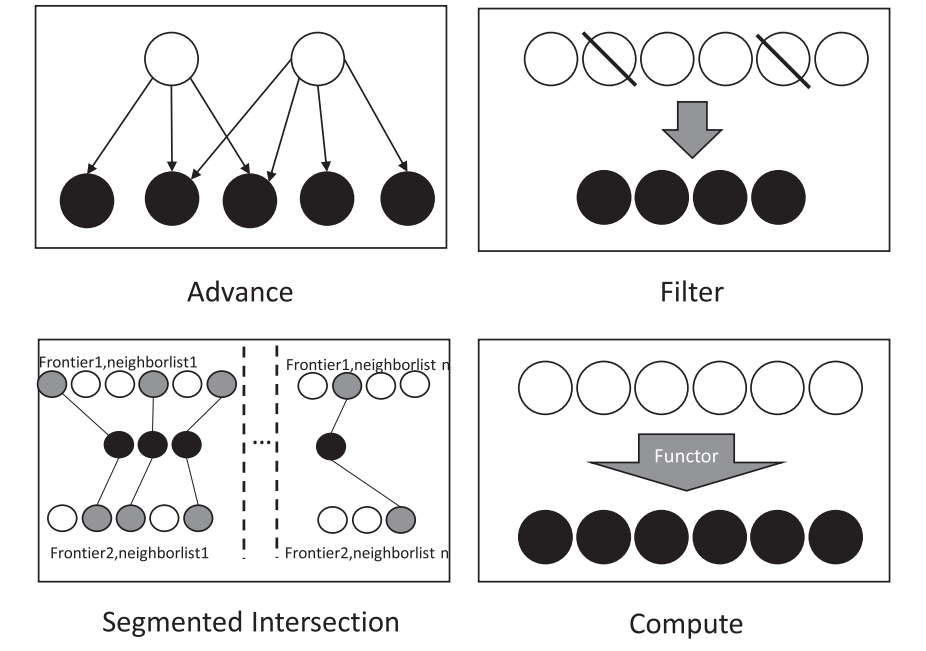
\includegraphics[width=0.6\textwidth]{Chapters/Figures/Images/gunrock_ops_updated.png}
        \caption{Gunrock's operators. Input frontier in white/grey and output frontier in black (taken from~\cite{paper:gunrock}).}
    \label{fig:gunrockops}
    \end{figure}

    Gunrock offers one compute operator and three traversal operators: advance, filter, and segmented intersection. These operators can be visualized in Figure ~\ref{fig:gunrockops} and are defined as follows:

    \begin{itemize}
        \item \textbf{Advance:} An advance operator generates a new frontier from the input frontier by visiting its neighbors. Each input item maps to multiple output items from the input item’s neighbor list.
        \item \textbf{Filter:} A filter operator generates a new frontier from the input frontier by choosing a subset of the input frontier based on programmer-specified criteria. Each input item maps to zero or one output item.
        \item \textbf{Segmented Intersection:} A segmented intersection operator takes two input frontiers $F$ and $F'$ with the same length and generates both the number of total intersections and the intersected node IDs as the new frontier. The intersections are performed between the neighbors of all the pairs of vertices $(v_i, v'_i), v_i \in F \land v'_i \in F' \land i \in \{0, |F|\}$. The resulting frontier is the set of common neighbors between the pairs of vertices $(v_i, v'_i)$.
        \item \textbf{Compute:} A compute operator defines an operation to be applied on all elements of its input frontier. A programmer-specified compute operator can be used together with all three traversal operators.
    \end{itemize}
    
    A new graph primitive can be composed as a sequence of these four operators, which are then executed sequentially by Gunrock. It is often desired that primitives run to convergence. Gunrock generally expresses a convergence as an empty frontier. However, a developer can use different criteria, which can be specified using a computation operator.

    Gunrock stores per-vertex and per-edge data as a \gls{SOA}, allowing coalesced memory accesses. Both vertex-centric and edge-centric operations are supported. To achieve this. the graph is stored using a \gls{CSR} sparse matrix for vertex-centric operations by default, but users can also choose an edge-list-only representation for edge-centric operations.

    Gunrock shows better performance than other \gls{GPU}-based graph processing frameworks like MapGraph~\cite{paper:mapgraph} and CuSha~\cite{paper:cusha}, and competitive performance against nvGRAPH.

    % -----------

    \paragraph{\textbf{cuSTINGER}.}
    cuSTINGER~\cite{paper:custinger} is designed for streaming graphs that evolve over time. Contrary to static graph processing frameworks, which require the entire graph to be re-transmitted to the \gls{GPU} whenever an update is issued, cuSTINGER only transmits the updates themselves, which drastically decreases the amount of memory being transferred. The \gls{GPU} then applies the update internally. cuSTINGER handles all the memory allocation, allowing the programmer to focus on designing the graph processing algorithms and not worrying about the implementation of the dynamic data structure. Even though cuSTINGER is mainly aimed at dynamic graphs, it also supports static graph processing. Multiple memory allocators, which influence the amount of memory being allocated for each vertex, are provided. When dealing with static graphs, a compact memory allocator can be chosen. For dynamic graphs, another allocator can be chosen that trades memory usage for better update performance.
    
    %cuSTINGER is a \gls{GPU} extension of the \gls{STINGER} data structure discussed in section~\ref{graph_data_structures}.
    cuSTINGER is a \gls{GPU} extension of the \gls{STINGER} data structure. \gls{STINGER}'s layout is based on the blocked adjacency lists data structure discussed in section~\ref{graph_data_structures}.
    In cuSTINGER, the lists of edge blocks (per vertex) are replaced with a single adjacency array (per vertex). This allows for better edge locality within an adjacency list, for better memory utilization, and only requires one memory allocation per adjacency list (allows for a more efficient memory manager). When the arrays are allocated, some extra space is left for future inserts. cuSINGER takes advantage of an advanced memory manager that minimizes the number of calls made to the system memory allocation and deallocation functions, and groups adjacency lists into large chunks for better locality.
    
    The following graph update operators are supported: edge insertion, edge deletion, vertex insertion, and vertex deletion. Given that the \gls{GPU} is a highly parallel system, Oded Green and David A. Bader recommend that updates be grouped into batches.

    Since 2017, cuSTINGER has been superseded by Hornet.

    % -----------
    \paragraph{\textbf{Hornet}.}
    Hornet~\cite{paper:hornet} is a graph framework/data structure designed for dynamic sparse graphs and matrices. It is scalable with the input size and doesn't require memory re-allocation when updates are issued. Compared to aimGraph~\cite{paper:aimgraph} and cuSTINGER~\cite{paper:custinger}, it provides better memory usage, faster initialization, and faster updates. It only requires about 5\% to 25\% additional memory when compared to \gls{CSR}, and outperforms Gunrock~\cite{paper:gunrock} in a suite of algorithmic benchmarks.

    Hornet is composed of two layers, a user interface and an internal representation abstracted from the user. From the user's perspective, each vertex has two associated fields: the number of neighbors, and an adjacency list that references those neighbors.
    
    To ensure fast updates, Hornet does not use the standard memory allocation function. Instead, a data manager implements this function with the usage of three data structures: 1) Block arrays that store adjacency lists, 2) A vectorized bit tree that can efficiently reclaim empty blocks, and 3) A B+Tree to manage the block-arrays. A block-array is simply an array composed of equally sized chunks. The vectorized bit tree is used to find empty blocks within block-arrays at high rates. It does so by using a simple and fast lookup strategy. cuSTINGER on the other hand, requires computationally intensive searches for this purpose. The B+Tree is responsible for finding block-arrays that have free blocks. Each node of a B+Tree is a tuple <data, key>. The data field points to the block-array and the key stores the number of free blocks in that block-array. Given that searches in such a tree take $log(t)$ time, and that the number of block-arrays of a given size is relatively small, it is able to execute these searches very fast.
    
    The following graph updates are supported: insertion and deletion of vertices, insertion and deletion of edges, and update of values of vertices and edges. Vertex insertions and deletions are expressed using sequences of edge insertions and deletions. Updates are grouped in batches to maximize throughput.

    \paragraph{\textbf{Dynamic Gunrock}.} 
    Muhammad A. Awad et al. \cite{paper:dynamic_graph_gpu} proposed a dynamic graph data structure that utilizes a hash table per vertex, each storing a vertex's adjacency list. The authors claim that with this approach it is possible to gain significant speedups both in insertion (3.4 - 14.8x faster) and deletion (7.8x times faster) rates when compared to other state-of-the-art solutions like Hornet~\cite{paper:hornet} and FaimGraph~\cite{paper:faimgraph}. This is achieved given hash tables' fast query rates and their ability to ensure uniqueness while performing updates. Regarding the "front-end", the framework is integrated into Gunrock~\cite{paper:gunrock}.

    % One of the main concerns when dealing with dynamic graphs, is deciding how to store the vertices' adjacency lists. The most straightforward approaches to store per-vertex adjacency lists are using a variable-sized list (like Hornet) or a list composed of fixed sized pages (like FaimGraph). However, the authors argue, that more sophisticated data structures like hash-tables or B-Trees can yield better results, allowing for high throughput of updates and lookups.

    The proposed data structure is composed of a vertex dictionary and a set of adjacency lists (stored using hash tables). The vertex dictionary is represented using a fixed-size array, where vertices are indexed by vertex ID. For the adjacencies, one hash table is used per vertex. Each hash table is composed of a set of buckets. To calculate the number of necessary buckets, a user defined load factor combined with the graph's connectivity information is used in order to reduce memory allocation overhead. Additionally, a dynamic memory allocator is used whenever new slabs need to be allocated as a hash table grows.

    The data structure is built on top of Slab Hash~\cite{paper:slablhash}, a dynamic hash-table for the \gls{GPU}. In order to ensure good performance, all operations are implemented using a \gls{WCWS} strategy. In \gls{WCWS}, each thread has an independent task assigned to it, but all threads within a warp cooperate with each other to collectively perform one independent task at a time. This type of strategy allows for \gls{GPU} optimized memory access patterns.

    Most graph updates only require appending or removing elements from the hash tables, allocating new slabs when needed. Vertex deletion requires a more sophisticated algorithm, given that it requires deleting all adjacencies that include the vertex at hand. To mitigate load imbalance, a queue is utilized to manage the deletion of vertices. 

    \paragraph{\textbf{FaimGraph}.}
    %
    FaimGraph~\cite{paper:faimgraph} is a fast fully dynamic graph framework developed by the same authors of aimGraph~\cite{paper:aimgraph}, improving on the previous work, and assessing its limitations. It achieves high update rates while keeping a low memory footprint by taking advantage of memory management directly on the \gls{GPU}. With this approach, it is possible to perform initialization in parallel (up to 300 times faster than previous work) and perform updates directly on the \gls{GPU}. Queuing techniques are also used to reclaim memory, reducing the memory footprint, and allowing for occasional faster inserts. Unlike other \gls{GPU} dynamic graph frameworks that only support edge insertions and deletions, like aimGraph~\cite{paper:aimgraph}, FaimGraph allows for fully dynamic graphs (vertex insertion and deletion).

    During initialization, FaimGraph allocates a single large memory block on the \gls{GPU}, to avoid \gls{CPU} round-trips, which is than managed by the framework's memory manager. This memory block is mostly composed of the queuing structures, vertex data, and edge data. It also keeps track of memory sections, graph properties, free pages, and unused indices. Figure~\ref{fig:faimgraph_data_structure} shows a visualization of the device memory layout.

    \begin{figure}[tbp]
        \centering
        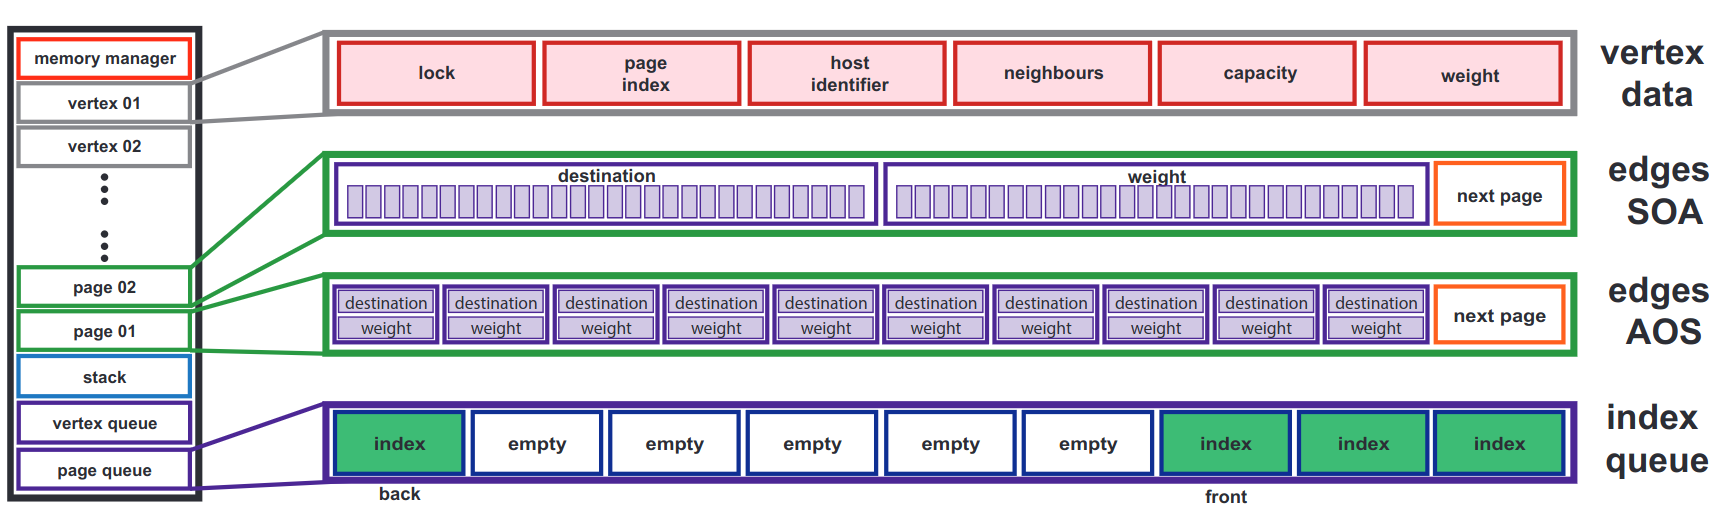
\includegraphics[width=1.0\textwidth]{Chapters/Figures/Images/faimgraph_ds.png}
        \caption{Faimgraph memory layout (taken from~\cite{paper:faimgraph}).}
        \label{fig:faimgraph_data_structure}
    \end{figure}

    As stated before, the main mechanism to reclaim memory uses a set of index queues. Whenever a vertex is deleted, its index is enqueued to the respective index queue. The same applies, whenever an adjacency page is deleted. During resource allocation, threads first try to dequeue a deleted index. If successful, the memory relative to the index is reclaimed, otherwise, the vertex or page region is increased.

    Vertex data is stored as a dynamically growing array of structures. The number of attributes for each vertex isn't limited, given that the memory manager can adapt to any vertex size. Storing vertices contiguously in this manner allows for coalesced memory accesses and simple indexing. Additionally, the vertex identifier used on the \gls{CPU} is mapped to the device identifier. Edges are stored as a linked list of fixed-sized pages of edges. A larger page size allows for more efficient traversal, while small pages allow for less memory fragmentation and allocation overhead. A page size of 64 bytes was chosen by the authors.

    Both vertex and edge insertions and deletions are performed as expected. Appending and removing values from the data structures, increasing the vertex or page regions when needed, and reclaiming memory using the index queues as discussed before. Shuffle operations are also utilized to ensure sorting order when performing updates.
    % One relevant implementation detail lies in the method of performing edge deletions efficiently. When removing an edge from the middle of the adjacency list, instead of moving all the following edges to the left (a costly operation), the last edge from the list is moved to fill the gap left by the deleted edge.

    According to the authors, FaimGraph outperforms multiple state-of-the-art frameworks, including Hornet~\cite{paper:hornet}, aimGraph~\cite{paper:aimgraph}, cuSTINGER~\cite{paper:custinger} and GPMA~\cite{paper:gpma}, in a suit of benchmarks that test initialization times, graph update rates and algorithmic performance.


    \paragraph{\textbf{Previous Marrow-Graph}.}
    %    
    Previous work~\cite{marrow_graph} has already studied the feasibility of developing a dynamic graph data structure and framework using Marrow (with an OpenCL backend). In this section, we provide a brief overview of the implementation and features of the previously developed Marrow-Graph.
    
    The chosen data structure to store graphs was slotted pages~\cite{paper:turbograph} (discussed in greater detail in section~\ref{sec:graph_data_structures}) represented using marrow containers. 
    %A marrow array is stored both on the host and device, and Marrow handles any necessary synchronization. 
    The graph is stored using a set of fixed-sized slotted pages, each represented as a marrow array. Each slotted page stores the attributes of a set of vertices and their respective adjacency lists. Besides the slotted pages, two auxiliary data structures are used. One to keep track of large adjacency lists, represented as a marrow vector, and another, which is only present on the \gls{GPU}, to store the device addresses of each slotted page.
    
    Graph manipulations are performed on the \gls{CPU}. The data structure is updated on the host and later synchronized to the device automatically by Marrow in a lazy manner. Edge insertions are performed by inserting the new edge in the respective slotted page. If the slotted page is full, a new one is allocated and marked as a large adjacency list. Vertex insertions are implemented by appending a new vertex to the last slotted page. If the last slotted page is full, a new one is allocated. Deletions follow a similar logic (if a page becomes empty, it is deleted), however, vertex deletions bring the added complexity of needing to delete all edges that include the deleted vertex. It should be noted that these manipulations can often result in reallocations, but only inside a given slotted page. This means that if the size of the pages is kept "small", the reallocations do not involve a large number of elements.
    
    For graph processing, the solution uses the same set of primitives defined by Gunrock~\cite{paper:gunrock}: compute, advance, filter, and segmented intersection. These operations are further discussed in section~\ref{sec:graph_data_structures}. All of these operations were implemented using preexisting marrow functions combined with custom OpenCL functions, defined over marrow containers. With these basic operations, it is possible to implement practically all major graph processing algorithms. Because of time constraints, however, only \gls{BFS} and \gls{SSSP} were implemented. Another limitation found, is the inability to combine the compute operator with the other three, as proposed by Gunrock.

    Regarding the performance of the manipulation operations, the construction of the graph can not be properly accelerated due to the nature of the slotted pages data structure and its representation using Marrow. Deletions are accelerated through the use of a range function. Insertions are relatively costly but do not require any previous knowledge about the number of vertices and edges.

    When compared to Gunrock, Marrow-Graph shows competitive performance in the \gls{BFS} benchmarks when considering the time of the graph construction plus the time of the algorithm's execution time, but falls behind when discarding graph construction time. Compared to Hornet~\cite{paper:hornet}, it shows significantly slower execution times in all benchmarks. The author explains that Marrow-Graph is slower in most benchmarks due to the significant overhead associated with the advance operator to locate vertices in the correct pages. Another factor is related to the usage of OpenCL, while other frameworks, like Hornet and Gunrock, are implemented using \gls{CUDA}, which is optimized to offer better performance with Nvidia graphics cards.

    \begin{table}[]
        \centering
        \small
        \begin{tabular}{| c | c c c c c |}
            \hline
            Framework &  \makecell{Intended \\ Hardware} & \makecell{Internal \\ Data Structure} & Dynamic & Unit & \makecell{Programming \\ Model} \\
            \hline
            \hline
            % \gls{GPU}
            Gunrock &  GPU & CSR or Other &  & VEC & BSP \\
            D. Gunrock & GPU & Vector of HTs & \checkmark & VEC & BSP \\
            Hornet & GPU & Adjacency Lists \& Trees & \checkmark & VC & BSP  \\
            CuSTINGER &  GPU & STINGER & \checkmark & VC & BSP \\
            FaimGraph & GPU & Blocked Adjacency Lists & \checkmark & VC &  BSP\\
            CuSha &  GPU & G-Shards and CWs &  & VC & BSP \\
            MapGraph &  GPU & CSR &  & VC & BSP \\
            %Frog &  GPU & CSR &  & VC & \\
            Medusa &  GPU & Custom &  & VEC & BSP \\
            % Shared Memory
            LLAMA &  MC CPU & CSR-Like & \checkmark & VC & - \\
            GraphLab & MC CPU & CSR-Like & \checkmark & VC & -  \\ % data structure: SGraph
            Ligra & MC CPU & CSR-Like &  & VC & - \\
            Ringo & MC CPU & HT of Vectors & \checkmark & VC & - \\
            Polymer & MC CPU & CSR-Like &  & VC & - \\
            
            % GraphMat & Multi-Machine & Adjacency Matrix ? & N.D \\
            % HPC
            % PBGL & Multi-Machine & Adjacency List & \checkmark & VC \\
            % CombBLAS & Multi-Machine & Adjacency Matrix & \checkmark & EC \\
            % %HavoqGT & Multi-Machine & Dist. Edge Lists & \checkmark \\
            % % Dist.
            GraphIn & Cluster & CSR \& Edge Lists & \checkmark & VC & I-GAS \\
            Chaos & Cluster & Edge-List &   & EC & Scatter-Gather \\
            PowerGraph & Cluster & CSR-Like & \checkmark & VC & GAS \\
            GraphX & Cluster & Spark RDD & \checkmark & VC & BSP \\
            Pregel & Cluster & Adjacency Lists &  & VC & GAS \\
            
            \hline
        \end{tabular}
        \caption{Graph processing frameworks
        %N.D.: Not Determined; 
        (MC: Multi-Core, VC: Vertex-Centric, EC: Edge-Centric, VEC: Vertex \& Edge-Centric, HT: Hash-Table).}
        \label{tab:graph_processing_frameworks}
    \end{table}

    \begin{table}[]
        \small
        \centering
        \begin{tabular}{| c | c c c c c c c |}
            \hline
            Framework & \makecell{Public \\ Repository} & \makecell{Compiles\\ \& Runs} & Directed & Weighted & \makecell{VVEA} & Language & FDP \\
            \hline
            \hline
            Gunrock & \checkmark &\checkmark & \checkmark & \checkmark &  & \gls{CUDA} &  \\
            D. Gunrock & \checkmark &  & \checkmark & \checkmark &  & \gls{CUDA} & \checkmark \\
            Hornet & \checkmark & \checkmark & \checkmark & \checkmark &  & \gls{CUDA} & \\
            FaimGraph & \checkmark & \checkmark & \checkmark & \checkmark & \checkmark & \gls{CUDA} & \checkmark \\
            \hline
        \end{tabular}
        \caption{\gls{GPU}-Accelerated graph processing competitors (VVEA: Variable Vertex and Edge Attributes, FDP: Full Dynamic Processing).}
        \label{tab:gpu_graphs}
    \end{table}

    \subsection{Conclusions}
    The potential competitors (the ones we will evaluate against) to our solution are found in Table~\ref{tab:gpu_graphs}. Currently we will only consider \gls{GPU}-based solutions, but distributed solutions can also be relevant for future work that explores multi-\gls{GPU} systems. Gunrock is the state-of-the-art static \gls{GPU}-accelerated graph processing framework, so even though it is not a direct competitor, considering it only supports static graphs, it can be used as a baseline for algorithmic performance evaluation. Regarding its dynamic counterpart~\cite{paper:dynamic_graph_gpu}, we were not able to successfully compile its publicly available implementation (found on Github as a branch in Gunrock's repository). For our direct competitors, this leaves us with Hornet and FaimGraph. cuSTINGER is not considered since it has been superseded by Hornet. All three competitors Gunrock, Hornet, and FaimGraph, are directed, weighted and are implemented using \gls{CUDA}. FaimGraph, contrary to the other frameworks, allows for user-defined vertex and edge attributes. This can be useful for more specialized graphs. Another noteworthy observation is that even though Hornet supports \gls{GPU}-accelerated processing over dynamic graphs, only a small number of algorithms have actually been implemented to run on the fully dynamic data structure.


% weighted / direction / multi-GPU



% Conclusions: 
% - Which data structure (talk about compactness, performance and update-friendliness)
% - Which programming model (talk about performance, V.C. vs E.C. and modularity / ease of use for writing algorithms)
% - 


% cpu based:
%     - llama (relevant)
%     - graphlab (important but discontinued)
%     - ligra (maybe ignore)
%     - ringo (intersting, hashtable of nodes, and dynamic)
%     - polymer (interesting NUMA aware and dynamic. Not very known. Maybe ignore)
%     - BGL?
%     - SNAP?

% papers to read:

%     LLAMA
%     GraphLab
%     RINGO
%     BGL
%     SNAP
    